% !TeX root = tfm.tex
\documentclass[a4paper,11pt]{report}
%\documentclass[a4paper,twoside,11pt,titlepage]{book}
\usepackage{listings}
\usepackage[utf8]{inputenc}


% \usepackage[style=list, number=none]{glossary} %
%\usepackage{titlesec}
%\usepackage{pailatino}

\usepackage{dcolumn}
\newcolumntype{.}{D{.}{\esperiod}{-1}}
\makeatletter
\makeatother


%\usepackage[chapter]{algorithm}
%\RequirePackage{verbatim}
%\RequirePackage[Glenn]{fncychap}
\usepackage[dvipsnames]{xcolor}
\usepackage{fancyhdr}
\usepackage{graphicx}
\usepackage{afterpage}
\usepackage{cite}
\usepackage{longtable}
\usepackage{amsmath}
\usepackage{subfigure}
\usepackage{listings}
\usepackage{multirow}
\usepackage{eurosym}
\usepackage{notoccite}
\usepackage[bookmarks = true, colorlinks=true, linkcolor = black, citecolor = black, menucolor = black, urlcolor = black]{hyperref}

%\usepackage[pdfborder={000}]{hyperref} %referencia

% ********************************************************************
% Re-usable information
% ********************************************************************
\newcommand{\myTitle}{Título del proyecto\xspace}


%\hyphenation{}

%\usepackage{doxygen/doxygen}
\usepackage{pdfpages}
\usepackage{url}
\usepackage{colortbl,longtable}
\usepackage[stable]{footmisc}
\usepackage{index}

%\makeindex
%\usepackage[style=long, cols=2,border=plain,toc=true,number=none]{glossary}
% \makeglossary

% Definición de comandos que me son tiles:
%\renewcommand{\indexname}{Índice alfabético}
%\renewcommand{\glossaryname}{Glosario}

\pagestyle{fancy}
\fancyhf{}
\fancyhead[LO]{\leftmark}
\fancyhead[RE]{\rightmark}
\fancyhead[RO,LE]{\textbf{\thepage}}
\renewcommand{\chaptermark}[1]{\markboth{\textbf{#1}}{}}
\renewcommand{\sectionmark}[1]{\markright{\textbf{\thesection. #1}}}

\setlength{\headheight}{1.5\headheight}

\newcommand{\HRule}{\rule{\linewidth}{0.5mm}}
%Definimos los tipos teorema, ejemplo y definición podremos usar estos tipos
%simplemente poniendo \begin{teorema} \end{teorema} ...
\newtheorem{teorema}{Teorema}[chapter]
\newtheorem{ejemplo}{Ejemplo}[chapter]
\newtheorem{definicion}{Definición}[chapter]

\definecolor{gray97}{gray}{.97}
\definecolor{gray75}{gray}{.75}
\definecolor{gray45}{gray}{.45}
\definecolor{gray30}{gray}{.94}
\definecolor{codegreen}{rgb}{0,0.6,0}
\definecolor{codegray}{rgb}{0.5,0.5,0.5}
\definecolor{codepurple}{rgb}{0.58,0,0.82}
\definecolor{backcolour}{rgb}{0.95,0.95,0.92}


\lstdefinestyle{Python}{
	backgroundcolor=\color{backcolour},   
	commentstyle=\color{codegreen},
	keywordstyle=\color{magenta},
	numberstyle=\tiny\color{codegray},
	stringstyle=\color{codepurple},
	basicstyle=\scriptsize\ttfamily,
	breakatwhitespace=false,         
	breaklines=true,                 
	captionpos=b,                    
	keepspaces=true,                 
	numbers=left,                    
	numbersep=5pt,                  
	showspaces=false,                
	showstringspaces=false,
	showtabs=false,                  
	tabsize=2
} 

\usepackage{listings}
\usepackage{xcolor}
\usepackage{float}

\definecolor{eclipseStrings}{RGB}{42,0.0,255}
\definecolor{eclipseKeywords}{RGB}{127,0,85}
\colorlet{numb}{magenta!60!black}

\lstdefinelanguage{json}{
    basicstyle=\normalfont\ttfamily,
    commentstyle=\color{eclipseStrings}, % style of comment
    stringstyle=\color{eclipseKeywords}, % style of strings
    numbers=left,
    numberstyle=\scriptsize,
    stepnumber=1,
    numbersep=8pt,
    belowskip=1em,
	aboveskip=2em,
    showstringspaces=false,
    breaklines=true,
    string=[s]{"}{"},
    comment=[l]{:\ "},
    morecomment=[l]{:"},
    literate=
        *{0}{{{\color{numb}0}}}{1}
         {1}{{{\color{numb}1}}}{1}
         {2}{{{\color{numb}2}}}{1}
         {3}{{{\color{numb}3}}}{1}
         {4}{{{\color{numb}4}}}{1}
         {5}{{{\color{numb}5}}}{1}
         {6}{{{\color{numb}6}}}{1}
         {7}{{{\color{numb}7}}}{1}
         {8}{{{\color{numb}8}}}{1}
         {9}{{{\color{numb}9}}}{1}
}


\newcommand\YAMLcolonstyle{\color{red}\mdseries}
\newcommand\YAMLkeystyle{\color{black}\bfseries}
\newcommand\YAMLvaluestyle{\color{blue}\mdseries}

\makeatletter

% here is a macro expanding to the name of the language
% (handy if you decide to change it further down the road)
\newcommand\language@yaml{yaml}

\expandafter\expandafter\expandafter\lstdefinelanguage
\expandafter{\language@yaml}
{
  keywords={true,false,null,y,n},
  basicstyle=\normalfont\ttfamily,                             % assuming a key comes first
  sensitive=false,
  comment=[l]{\#},
  morecomment=[s]{/*}{*/},
  commentstyle=\color{purple}\ttfamily,
  stringstyle=\YAMLvaluestyle\ttfamily,
  numbers=left,
numberstyle=\scriptsize,
stepnumber=1,
numbersep=8pt,
belowskip=1em,
aboveskip=2em,
showstringspaces=false,
breaklines=true,
  moredelim=[l][\color{orange}]{\&},
  moredelim=[l][\color{magenta}]{*},
  moredelim=**[il][\YAMLcolonstyle{:}\YAMLvaluestyle]{:},   % switch to value style at :
  morestring=[b]',
  morestring=[b]",
  literate =    {---}{{\ProcessThreeDashes}}3
                {>}{{\textcolor{red}\textgreater}}1
                {|}{{\textcolor{red}\textbar}}1
                {\ -\ }{{\mdseries\ -\ }}3,
}

% switch to key style at EOL
\lst@AddToHook{EveryLine}{\ifx\lst@language\language@yaml\YAMLkeystyle\fi}
\makeatother

\newcommand\ProcessThreeDashes{\llap{\color{cyan}\mdseries-{-}-}}

\setlength{\parskip}{\baselineskip}%
\setlength{\parindent}{0pt}%

% minimizar fragmentado de listados
\lstnewenvironment{listing}[1][]
   {\lstset{#1}\pagebreak[0]}{\pagebreak[0]}

\lstset{style=Python}

\setlength{\parindent}{0cm}

\newcommand{\bigrule}{\titlerule[0.5mm]}


%Para conseguir que en las páginas en blanco no ponga cabecerass
\makeatletter
\def\clearpage{%
  \ifvmode
    \ifnum \@dbltopnum =\m@ne
      \ifdim \pagetotal <\topskip
        \hbox{}
      \fi
    \fi
  \fi
  \newpage
  \thispagestyle{empty}
  \write\m@ne{}
  \vbox{}
  \penalty -\@Mi
}
\makeatother

\usepackage{pdfpages}


\begin{document}
%\pdfbookmark[-1]{Memoria proyecto}{}
\begin{titlepage}


\newlength{\centeroffset}
\setlength{\centeroffset}{-0.5\oddsidemargin}
\addtolength{\centeroffset}{0.5\evensidemargin}
\thispagestyle{empty}

\noindent\hspace*{\centeroffset}
\begin{minipage}{\textwidth}

\centering

\includegraphics[scale=0.6]{imagenes/upm.png}\\[1.4cm]

\textsc{ Universidad Politécnica de Madrid\\[0.2cm]}
\textsc{ \Large TRABAJO FIN DE MASTER\\[0.2cm]}

% Upper part of the page
%
% Title
{\Large \bfseries  Desarrollo y despliegue de un sistema descentralizado y escalable de predicción orientado a Smart Cities utilizando técnicas de aprendizaje automático y datos abiertos.\\
}
%\noindent\rule[-1ex]{\textwidth}{3pt}\\[3.5ex]
\end{minipage}

\vspace{2cm}
\noindent\hspace*{\centeroffset}\begin{minipage}{\textwidth}
\centering

\textbf{Autor}\\ {Jose Antonio Hurtado Morón}\\[2.5ex]
\textbf{Tutor}\\ {Jose Andrés Muñoz Arcentales}\\[2ex]
\textbf{Ponente}\\{Ángel Palomares Caballero}\\[2cm]
%\includegraphics[width=0.3\textwidth]{imagenes/etsiit_logo.png}\\[0.1cm]
\textsc{Máster Universitario en Ingeniería de Redes y Servicios Telemáticos}\\[1cm]
\textsc{---}\\
Madrid, Enero 2022
\end{minipage}
%\addtolength{\textwidth}{\centeroffset}
%\vspace{\stretch{2}}
\end{titlepage}



\begin{titlepage}



\setlength{\centeroffset}{-0.5\oddsidemargin}
\addtolength{\centeroffset}{0.5\evensidemargin}
\thispagestyle{empty}

\noindent\hspace*{\centeroffset}
\begin{minipage}{\textwidth}

\centering

\includegraphics[scale=0.6]{imagenes/upm.png}\\[1.4cm]

\textsc{ Universidad Politécnica de Madrid\\[0.2cm]}
\textsc{ \Large TRABAJO FIN DE MASTER\\[0.2cm]}

% Upper part of the page
%
% Title
{\Large \bfseries  Desarrollo y despliegue de un sistema descentralizado y escalable de predicción orientado a Smart Cities utilizando técnicas de aprendizaje automático y datos abiertos.\\
}
%\noindent\rule[-1ex]{\textwidth}{3pt}\\[3.5ex]
\end{minipage}

\vspace{2cm}
\noindent\hspace*{\centeroffset}\begin{minipage}{\textwidth}
\centering

\textbf{Autor}\\ {Jose Antonio Hurtado Morón}\\[2.5ex]
\textbf{Tutor}\\ {Jose Andrés Muñoz Arcentales}\\[2ex]
\textbf{Ponente}\\{Alonso Gonzalez Álvaro}\\[2cm]
\textit{Departamento de Ingeniería de Sistemas Telemáticos} \\
%\includegraphics[width=0.3\textwidth]{imagenes/etsiit_logo.png}\\[0.1cm]
\textsc{Máster Universitario en Ingeniería de Redes y Servicios Telemáticos}\\[1cm]
\textsc{---}\\
Madrid, Enero 2022
\end{minipage}
%\addtolength{\textwidth}{\centeroffset}
%\vspace{\stretch{2}}
\end{titlepage}



%\begin{titlepage}



\setlength{\centeroffset}{-0.5\oddsidemargin}
\addtolength{\centeroffset}{0.5\evensidemargin}
\thispagestyle{empty}

\noindent\hspace*{\centeroffset}
\begin{minipage}{\textwidth}

\centering

\includegraphics[scale=0.6]{imagenes/upm.png}\\[1.4cm]

\textsc{ Universidad Politécnica de Madrid\\[0.2cm]}
\textsc{ \Large TRABAJO FIN DE MASTER\\[0.2cm]}

% Upper part of the page
%
% Title
{\Large \bfseries  Desarrollo y despliegue de un sistema descentralizado y escalable de predicción orientado a Smart Cities utilizando técnicas de aprendizaje automático y datos abiertos.\\
}
%\noindent\rule[-1ex]{\textwidth}{3pt}\\[3.5ex]
\end{minipage}

\vspace{2cm}
\noindent\hspace*{\centeroffset}\begin{minipage}{\textwidth}
\centering

\textbf{Autor}\\ {Jose Antonio Hurtado Morón}\\[2.5ex]
\textbf{Tutor}\\ {Jose Andrés Muñoz Arcentales}\\[2ex]
\textbf{Ponente}\\{Alonso Gonzalez Álvaro}\\[2cm]
\textit{Departamento de Ingeniería de Sistemas Telemáticos} \\
%\includegraphics[width=0.3\textwidth]{imagenes/etsiit_logo.png}\\[0.1cm]
\textsc{Máster Universitario en Ingeniería de Redes y Servicios Telemáticos}\\[1cm]
\textsc{---}\\
Madrid, Enero 2022
\end{minipage}
%\addtolength{\textwidth}{\centeroffset}
%\vspace{\stretch{2}}
\end{titlepage}



{\Large \bfseries Resumen}

La adopción cada vez más amplia por parte de entidades públicas y privadas de los Datos Abiertos o \textbf{Open Data}, abre la puerta a nuevos proyectos y desarrollos que hacen uso de estos en múltiples campos y contextos. \textbf{FiWare}, es una plataforma abierta focalizada en la gestión y consumo de datos para Smart Cities, y mediante su marco de herramientas de desarrollo nos permite integrar estos datos abiertos en sistemas a gran escala. Desplegar y administrar estas aplicaciones y sistemas a nivel de producción, incluso para configuraciones aparentemente simples, puede introducir enormes barreras de complejidad para los desarrolladores y científicos de datos, tanto por la cantidad de datos en tiempo real a procesar como por la complejidad que pueden adquirir estos sistemas a la hora de escalarlos. \textbf{Kubernetes} y \textbf{Spark}, entre otras tecnologías, nos proporcionan esta capa de abstracción a la hora de pensar en estos sistemas a gran escala, y hacen más fácil y rápido el tratamiento y mantenimiento de ellos.

El principal objetivo de este proyecto es el de demostrar el potencial de estas tecnologías por separado y en conjunto, que nos permiten automatizar y mejorar el despliegue de este tipo de entornos. Para ello, desarrollaremos un caso de uso que involucre todo el proceso: una aplicación web para la interacción con el usuario, una arquitectura en la nube basada en micro servicios y un modelo de predicción entrenado con datos recogidos en tiempo real, que permitan al usuario obtener una predicción de la ocupación de los aparcamientos públicos de su ciudad.\\

{\Large \bfseries Abstract}

The increasing adoption of \textbf{Open Data} by public and private entities opens the door to new projects and developments that make use of these huge amounts of data for multiple applications in several fields and contexts. \textbf{FiWare} is an open platform focused on the management and consumption of data for Smart Cities, and through its framework of development tools, allows us to integrate these unstructured open data in large-scale systems. Deploying and administrating these applications and systems at production level, even for seemingly simple configurations, can introduce huge barriers of complexity for developers and data scientists, both because of the amount of real-time data to be processed and the increasing complexity that these systems can acquire when scaling them out. \textbf{Kubernetes} and \textbf{Spark}, among other technologies, provide us with this layer of abstraction when thinking about these large-scale systems, and make it easier and faster to process and maintain them.

The main goal of this project is to show the potential of these technologies both separately and together, allowing us to automate and improve the deployment of this kind of environment. To do so, we will design a use case that involves the whole process: a web application for user interaction, a cloud architecture based on micro-services, and a prediction model trained with open data, collected in real-time from a public data source, that will allow the user to obtain a prediction of the occupancy of the public parking spaces in his city on a given date and time.

\textit{\textbf{Palabras clave / Key words: } Open Data, Smart Cities, Ciudades Inteligentes, IoT, FIWARE, Spark, Kubernetes, Docker, Machine Learning, Predictive Analysis, Big Data. }
%\pdfbookmark[0]{Índice}{}
\tableofcontents
\listoffigures
\listoftables

% Ficheros con los contenidos

\chapter{Introduction}
\label{chapter:Introduction}

\section{Motivation}
\label{section:Motivation}

\begin{figure}[h]
	\centering
	%\includegraphics[width=1\linewidth]{imagenes/ABSORCIONES.PNG}
	\caption{from \cite{}.}
	\label{LABEL}
\end{figure}

\section{Goals/Objectives}

\begin{itemize}
    \item A
    \item B
    \item C
\end{itemize}

\section{Structure}

\begin{itemize}
    \item At section \ref{chapter:Introduction} we discuss \textbf{Item} where.
\end{itemize}




\chapter{State of Art}
\label{chapter:StateOfArt}

\section{Open Data}
\label{section:OpenData}

Both public and private sectors produce a wide variety of information of interest for citizens and businesses, such as social, economic, geographic, statistical, meteorological, tourism, business and education information. This data has characteristics that make it particularly attractive to the digital content sector, as it is complete, reliable, and of high quality. There are many areas where we can expect this data to be valuable, and where examples of how it has been used already exist. Many different groups of people and organizations can also benefit from the availability of open data, including the public administrations themselves, but at the same time, it is impossible to predict precisely how and where value will be created in the future.

The openness of public sector data allows any person or organization to build on it a new idea that results in new data, knowledge, improve processes, add value to existing ones or even create new services. Consequently, it has considerable economic potential and also favors transparency, participation and citizen collaboration, which are necessary for a more open government.

Open data is data that can be freely used, re-used, and redistributed by anyone - subject only, at most, to the requirement to attribute and share-alike\cite{OpenDataHandbook}.

\subsection{Defining Open}

This paradigm of widely available data has been around since the first years of the internet, with open software in the lead and with the comprehension from most of the entities that form the web, that the share of knowledge always leads to improvements in the common future.

The word Open encompasses a wide range of definitions and nuances, but in this case, when we talk about open knowledge, it is important to correctly define what we are really referring to.

“Open means anyone can freely access, use, modify, and share for any purpose (subject, at most, to requirements that preserve provenance and openness).” \cite{what-is-open}

\subsection{Open Smart Cities}

While massive data collection through sensors attached to physical infrastruc-tures (or Big Data) had always been a characteristic feature of first-generation smart cities, publishing such data as open data or integrating with the open data published by city authorities on different aspects of city management and life is a relatively recent phenomenon. Actually, one of the main concerns related with the opening of data is individual privacy \cite{CONRADIE2014S10}, but this has been overcome in many ways. 

This seemingly shallow change can open the door for a great number of innovations, and lead to projects that could change how we live and interact with the cities themselves. Despite the short history of open data, there is evidence that it can significantly contribute to open government and transparency, citizens engagement, better-informed decisions,better services, innovative applications, and consequently new businesses and jobs.

Publishing Open Data extracted from different sources like traffic, pollution (not only air pollution, but also acoustic or luminous), public transport services use, affluence of popular public zones, etc, can lead to new solutions developed by individuals or companies, and also new material to research for academics, and consequently, have a positive impact in the city and the life of its inhabitants \cite{ojo2015tale}.

\subsection{Linked Data}

The term "Linked Data" refers to a set of best practices for publishing and connecting structured data on the Web. The web was built with the “Linked” concept from the beginning, with the creation of HTML and the “web” as we know it. However, in recent years the Web has evolved from a global information space of linked documents to one where both documents and data are linked \cite{bizer2011linked}.
Linked data is a set of best practices for ensuring that all data attributes can be easily compared when coming from a multitude of separate data sources, which could have a different idea as to what each attribute means. For example, when two data entities have a name attribute how can the computer be certain that it refers to a "Name of a thing" in the same sense. JSON-LD  introduces the concept of the context element, which provides additional information allowing the computer to interpret the rest of the data with more clarity and depth. But this doesn’t imply that this data should be freely accessible. That is where Open Linked Data comes in. 

Open Linked Data is data that the user can link from various sources, institutions, or organizations, and then explore and combine freely and without restrictions. It is also structured in an agreed format, as RFD, or JSON-LD, extended by NGSI-LD.

\clearpage

\section{Fiware}
\label{section:Fiware}

FIWARE \cite{fiware} is an open software platform promoted by the European ICT industry and the European Commission and developed inside the Future Internet Program (FI-PPP), that provides tools for developing smart solutions, and forms an innovation ecosystem for entrepreneurs to create new applications and services on the Internet. 

The FIWARE platform provides Smart Cloud capabilities, enhanced with a set of tools and libraries called Generic Enablers (GEs). These offer standardized and open APIs that facilitate tasks such as integrating Internet of Things devices, analyzing and processing medium and large scale data (Big Data), or incorporating advanced interfaces to interact with users. The generic enables provided by FIWARE can be classified into different categories, the most important being Context management, IoT, Robots and third-party systems, Context data processing, analysis and visualization, and Access management, publishing and monetization of APIs and context data.

\begin{figure}[H]
	\centering
	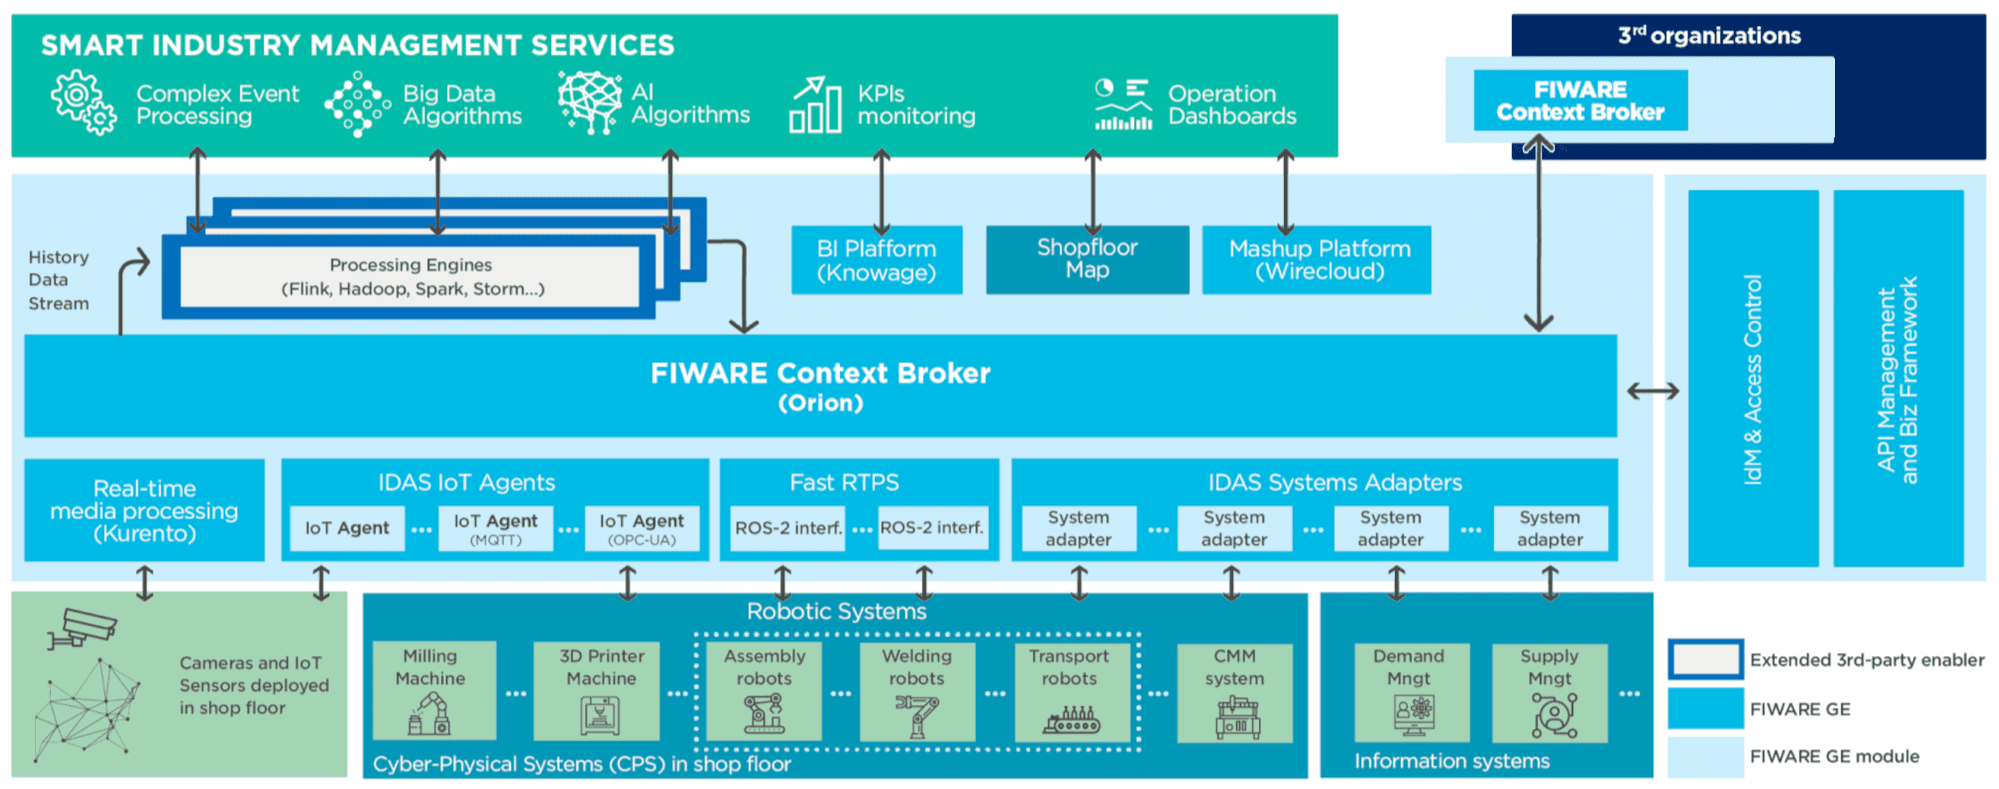
\includegraphics[width=1\linewidth]{imagenes/fiware-architecture.png}
	\caption{Diagram representing the main components of the FIWARE ecosystem. \cite{fiware-docs}}
	\label{fiware-architecture}
\end{figure}

Although FIWARE is a general-purpose platform, it is of special interest in the field of smart cities, due to the appropriateness of the technologies it provides and the importance of the innovation ecosystem in this environment. Since the beginning of the project, FIWARE has worked with a number of cities across Europe to validate and adapt its capabilities to the needs of a smart city, and functional platforms with a big IoT devices deployment has been executed in cities like Helsinki, Amsterdam, Torino, Lisbon, Santander, Seville, Málaga or Valencia between others.

When it comes to the publication and consumption of data, FIWARE  provides the \textbf{NGSI API}, which allows applications to make requests about the context and subscribe to changes in the context, which will be received through notifications. This is useful for example for real-time publication and consumption of sensor data or municipal services.

NGSI v2 is the new standard proposed by FIWARE to manage the context information, and in terms of the data model, properties can be seen as the combination of an attribute and its value. Relationships allow establishing associations between instances using linked data.

\begin{figure}[H]
	\centering
	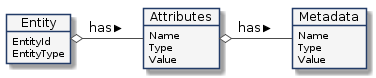
\includegraphics[width=0.8\linewidth]{imagenes/ngsi-v2.png}
	\caption{NGSIv2 entities schema. \cite{fiware-docs}}
	\label{ngsi-v2}
\end{figure}

The core element of NGSI v2 is the data entity, typically a real object with a changing state (such as a Room, a Building, and so on). Entities have attributes (such as name and temperature) and these, in turn, hold metadata such as a timestamp where the measure was taken. Every entity must have a type that defines the sort of thing the entity describes. Relationships can also be defined using NGSI v2, but only so far as giving the attribute an appropriate attribute name.

The core component of a FIWARE platform is the \textbf{Orion Context Broker}. Context information can come from many different sources: existing systems, users with a mobile application, sensor networks, etc. The Context Broker allows modeling and accessing context information regardless of the source of that information, and using its NGSI API, we can interact with the entities and subscriptions created inside it.

Another remarkable GE that we will use in this project is \textbf{Draco}, that is used to persist context data into third-party databases, creating a historical view of the context. It uses Apache NIFI in the background, and because of this, is really powerful for creating data pipelines from our Context Broker to our Database.

Besides the Context broker and Draco, most of the Generic Enablers provided by FIWARE acts as interfaces to hide the underlying complexity of the existing IoT protocols and adapt them to easily integrate with the platform.

\clearpage

\section{Kubernetes}
\label{section:Kubernetes}

Kubernetes \cite{kubernetes} was born as an internal container orchestration solution developed by Google. It is later presented as an open-source project in 2014, joined by large organizations such as Microsoft, Red Hat, IBM, Docker, Openshift, or Huawei.

Kubernetes has established itself as the leading container orchestrator. It allows orchestrating containers from a wide variety of different runtimes, not just Docker. In addition, some of the features that Kubernetes provides are a service discovery system, rollouts and rollbacks, resource optimization on nodes, secret configuration, horizontal scaling of our applications, and many more tools that allow huge and really optimized deployments on top of it. As a container orchestrator, it is designed to work in a declarative way, where instead of giving it the steps to reach a state, we indicate the state in which we want the service to deploy. An example of this is its management with the pods, minimal units of Kubernetes that will be discussed later, when one dies (event), it automatically raises another, provided it is indicated accurately enough.

Broadly speaking, the Kubernetes architecture is divided in two key elements, the master nodes, and the worker nodes. The master node is the entity that coordinates and manages the worker nodes in its cluster, where the containers run. , in the following diagram, the Kubernetes architecture is represented in more detail.


\begin{figure}[H]
	\centering
	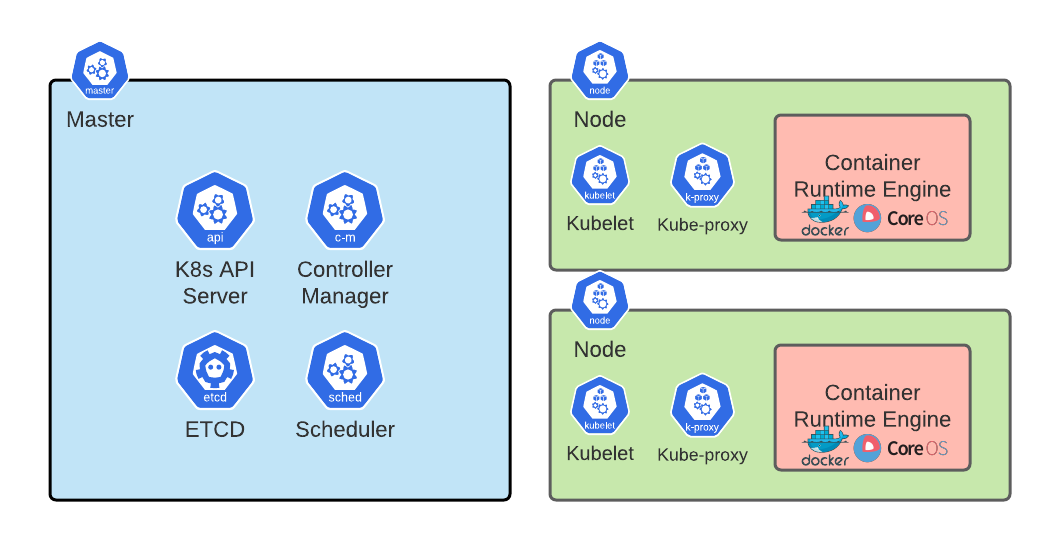
\includegraphics[width=1\linewidth]{imagenes/kubernetes-components.png}
	\caption{Kubernetes general architecture diagram.}
	\label{kubernetes-components}
\end{figure}

The main components of Kubernetes control plane \cite{cka-course}, represented in the previous diagram, have the following function:
\begin{itemize}
\item \textbf{ETCD}:  ETCD is a key-value store used by Kubernetes in order to store it's configuration and on-running information.

\item \textbf{Kube Controller Manager}: It manages the different controllers of Kubernetes. Controllers are like the brain of our cluster and are continuously monitoring the state of various components within the system, and working to maintain the desired functioning state of each one.

\item \textbf{Kube-Scheduler}: Primary management controller in Kubernetes. It manages the communication and management along the rest of the Kubernetes components, it is at the center of all the different tasks related to the cluster.

\item \textbf{Kube-API Server}: Decides which Pod goes on each Node. It doesn't place the pod on the Node though, this is the work of the kubelet of each node. The criteria used for this is based on certain condition: CPU Requirements, Memory resources, Rank function, labels, etc.

\item \textbf{Kubelet}: Kubelet is like the captain of each worker ship. It registers each node scheduled from the scheduler, creates the pods, and informs the master about the status and performance of each node. 

\item \textbf{Kube-proxy}: Pod networking solution to connect the Pods of the different nodes, making use of the Services. The Kube-proxy is a service that runs in each Worker node, and maintains an IP table of services, to route the connections of the different Pods, independently of the node.

\item \textbf{Pod}: A pod is a single instance of an application, and the smallest object that you can create in Kubernetes. A Pod usually contains a single container, and adds Kubernetes-related context to the actual container.
\end{itemize}

Besides the control components and the Pods, there are a lot of resources and objects that Kubernetes will put at our disposal to configure and deploy our applications on Kubernetes. Among them, we will use PersistentVolumes, Services, Deployments, StatefulSets, ReplicaSets or CronJobs.

Other tools designed to work with Kubernetes that we will use in this project are:

\textbf{Minikube}

Minikube \cite{minikube} is a tool created for deploying Kubernetes in your local machine. It uses Docker or any virtual machine environment to set up a single node cluster, this means that the control plane is in the same node that the application containers, but in a different namespace.

\textbf{Kubectl}

Kubectl is the command-line tool provided by Kubernetes to interact with our cluster. It allows us to inspect the cluster, create resources both in imperative and declarative mode.


\section{Machine Learning and Apache Spark}
\label{section:ML}

Machine learning is a branch of artificial intelligence that allows machines to learn without being specifically programmed to do so. By feeding the algorithm with data, it is able to recognize patterns and once trained, generate predictions on new data.

The original definition of Machine Learning, described it as “The field of machine learning is concerned with the question of how to construct computer programs that automatically improve with experience.” \cite{mitchell1997machine},but this definition is too generic, and nowadays with the great advances in both computation and applied statistics, the field has grown huge, we need to be more specific. For the scope of this project, we are not using models from several fields of the Machine Learning world, as Unsupervised Machine Learning or Deep Learning, so we will stick to this definition of the basic Supervised Machine Learning or Predictive modeling: “Find a model or procedure that makes best use of historical data comprised of inputs and outputs in order to skillfully predict outputs given new and unseen inputs in the future.” \cite{brownlee_2019}.

\subsection{Machine Learning Algorithms}

If we want to classify the most popular machine learning algorithms, we can group them by learning style or by similarity. By learning style, that means by how the interact with the input data, we can distinguish the Supervised, Semi-Supervised and Unsupervised categories.

\begin{itemize}
	\item \textbf{Supervised Learning}: Input data is called training data and has a known label or result such as spam/not-spam or a stock price at a time.
	\item \textbf{Unsupervised Learning}: Input data is not labeled and does not have a known result.
	\item \textbf{Semi-Supervised Learning}: Input data is a mixture of labeled and unlabelled examples.
\end{itemize}

\begin{figure}[H]
	\centering
	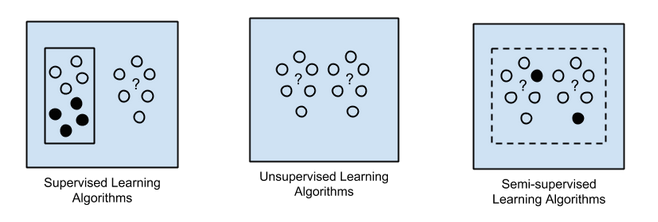
\includegraphics[width=1\linewidth]{imagenes/ml-algos.png}
	\caption{Main classification of ML algorithm by learning style.}
	\label{ml-algos}
\end{figure}

Algorithms related to Machine Learning are often also grouped by similarity in terms of their function (how they work). This generally seems like a more useful way of classifying them, because they also take into account the type of machine learning problem we are trying to solve (Regression and Classification).

Some of the more popular categories, with some examples, are: 

\begin{itemize}
	\item \textbf{Regression Algorithms:}:  They model the relationship between variables that is iteratively refined using a measure of the error in the predictions made by the model. (Linear Regressors, Logistic Regressors, Ordinary Least Squares Regression, etc).
	\item \textbf{Instance-based Algorithms}: Decision problem with instances or examples of training data that are deemed important or required to the model. (Kn-Neighbors, Locally Weighted Learning, Support Vector Machines)
	\item \textbf{Semi-Supervised Learning}: Input data is a mixture of labeled and unlabelled examples.
	\item \textbf{Decision Tree Algorithms}: These methods construct a model of decisions made based on actual values of attributes in the data. (Classification and Regression Tree, Decision Trees).
	\item \textbf{Artificial Neural Network and Deep Learning Algorithms}: These are models that are inspired by the structure and/or function of biological neural networks, and exploit abundant cheap computation. (Multi-Layer Perceptron, Stochastic Gradient Descent, Convolutional Neural Networks, Recurrent Neural Networks).
	\item \textbf{Ensemble Algorithms}: These are models composed of multiple weaker models that are 
	independently trained and whose predictions are combined in some way to make the overall prediction. (AdaBoost, Gradient Boosted Regression Trees, Random Forest).
\end{itemize}

Through the development of this project, we will some of these algorithms from different categories to compare which fits our problem and our data better.
 
\subsection{Apache Spark}

Apache Spark \cite{spark} is a programming framework for processing big data in a distributed manner, designed to be fast. Spark, unlike similar systems as Hadoop, doesn't store any data but loads them in memory for achieving a faster performance. This also makes Spark a really resource-consuming tool, and running it on top of Kubernetes is a good solution for making it more efficient.

Because it was created for being really good at performing tasks in parallel, it is usually deployed in a cluster mode, where a master node will run the main program and distribute the tasks on the worker nodes or executors. It includes APIs for Java, Scala, Python, and R and high-level tools like Spark SQL that allow working with all kinds of integrated functions and with good processing speeds.

The primary abstraction object provided by Spark is a resilient distributed dataset (RDD), which is a collection of partitioned elements between cluster nodes that can be operated on in parallel. RDDs are created by starting from a file or from an existing Scala collection in the driver program, and transforming it. Users can also ask Spark to persist an RDD in memory, allowing it to be efficiently reused through parallel operations, and convert them in DataFrames compatible with other use cases, like pandas DataFrames.

\begin{figure}[H]
	\centering
	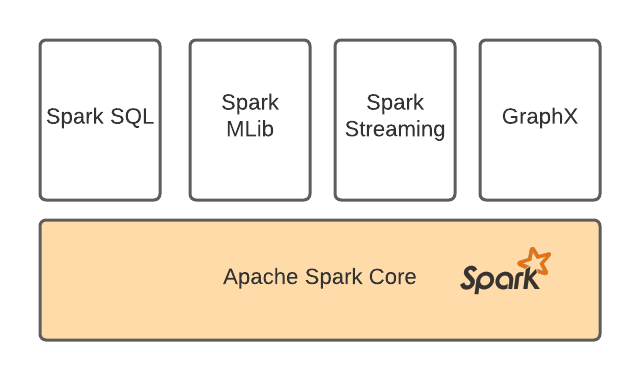
\includegraphics[width=1\linewidth]{imagenes/spark-core.png}
	\caption{Spark main modules and tools.}
	\label{spark-core}
\end{figure}

Some of the more popular tools in the Spark Environment, including the Spark Core itself, are:


\begin{itemize}
	\item \textbf{Spark Core}: This is the core of the Spark framework that supports the other modules.
	\item \textbf{Spark SQL}: Module for processing structured and semi-structured data.
	\item \textbf{MLlib}: Machine Learning library with various types of algorithms such as regression, classification, etc.
	\item \textbf{GraphX}: Graph processing (DAG).
	\item \textbf{Spark Streaming}: Real-time data processing.
\end{itemize}

In the development chapter (\ref{chapter:DesignAndImplementation}), we will explain in more detail how the Spark Cluster works and how to deploy applications on top of it.
\chapter{Motivation and Goals}
\label{chapter:Motivation}

With this project, our goal is to develop a scalable and microservices-based cloud system that will help us to create a complete platform oriented to smart cities. With this, we will be able to collaborate in the deployment and implementation of smart systems, focused on the cities in our area.

We will also collaborate with FIWARE on the adaptation of the platform to cloud environments such as Kubernetes and Spark, and in the future, it will be easily portable to any cloud service provider. With this, we will prove that scalable and modular deployments on the cloud can be achieved using FIWARE components and its Generic Enables, as well as other Open Source tools.

Collaterally, we will also help to make more useful and promote the use and publication of open data by public administrations and municipalities, and ultimately, we will try to improve the technological services offered to citizens, making available tools powered by the use of Machine Learning and the cloud.


\chapter{Design and implementation}
\label{chapter:DesignAndImplementation}
\section{Overview}
\label{section:Overview}

To approach the objectives of this project, we've focused on building a complete infrastructure based on microservices ready to be deployed on the cloud. In the course of this chapter, we will explain how we developed and configured several components, each one serving a  different task of our system.

Docker will help us to containerize each component and make it system-independent, and Kubernetes will help us orchestrate all the components and manage their scale and status. We will dedicate a subsection on each component to explain how we containerized and deployed it to the cluster. 

Inside Kubernetes, we will deploy these components:

\begin{itemize}
\item A web application where the users will be able to make predictions and interact with our system.
\item A MongoDB database to store all the raw and processed data.
\item Several FIWARE components that will enable the communication between our services, and manage the information context.
\item A Spark Cluster, that will run our machine learning model and process the data.
\item Other components to automate some tasks.
\end{itemize}

\begin{figure}[H]
	\centering
	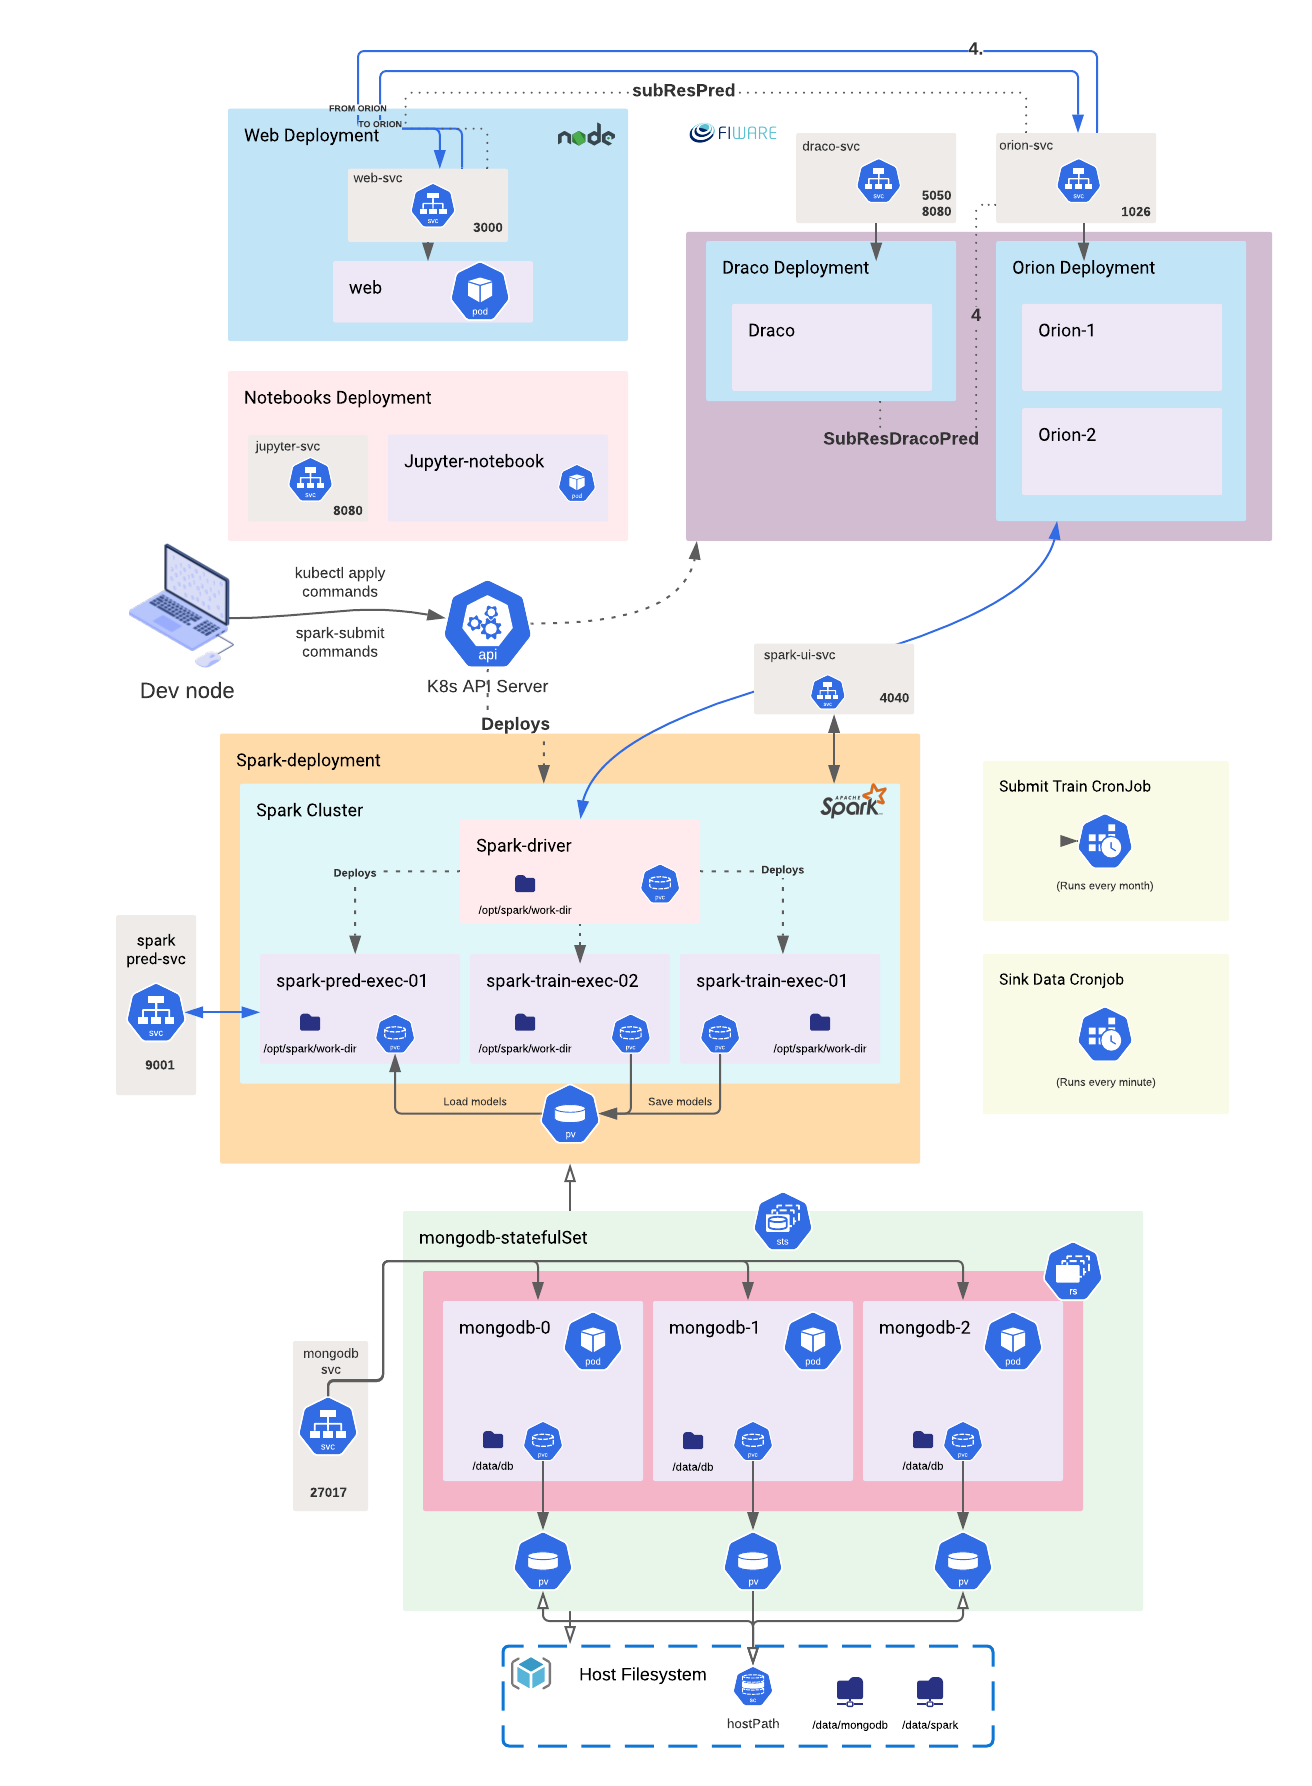
\includegraphics[width=1\linewidth]{imagenes/diagram.png}
	\caption{Representation of the Kubernetes architecture of the whole deployment.}
	\label{diagram}
\end{figure}

As cloud services providers like AWS or Google Cloud do not have free plans for a project with the resource requirements that Spark and Machine Learning add to our development,  we decided to use Minikube to host our Kubernetes cluster. Minikube is a single-node Kubernetes deployment focused on helping developers and administrators to set up a simple Kubernetes cluster in their local machine. Additionally, we will set up a docker registry in Docker Hub to store our images. 

Before going deeper into the development of the system, I would like to point out that all the code for this project is hosted in a Github Repository, and to replicate the cluster in another environment there is a dedicated script named \textit{create\_cluster.sh} that will do all the work. (\ref{CreateCluster})

\textit{Github repository}: https://github.com/tonihurtado/fiware-kube-ml-parking

\section{Web Application}
\label{section:WebApp}

The web application will be the interface for the users of the system, and it can also be seen as the starting point of the data flow.

\begin{figure}[H]
	\centering
	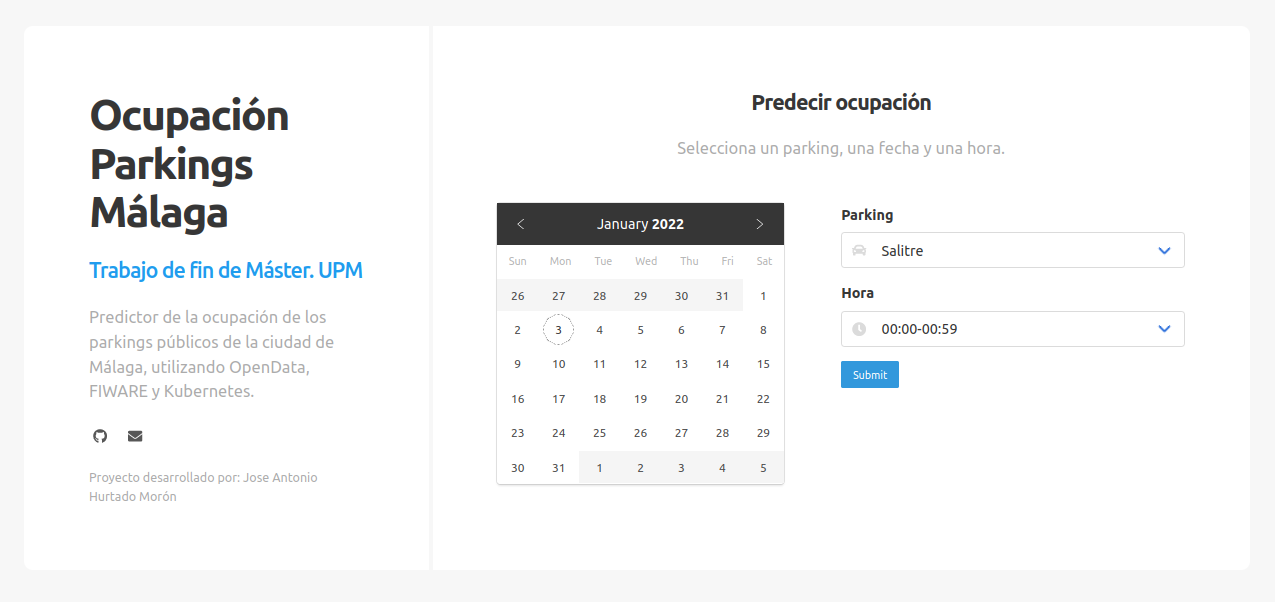
\includegraphics[width=1\linewidth]{imagenes/website.png}
	\caption{User Interface of the web application.}
	\label{website}
\end{figure}

The layout is simple, with a section on the left where the project is briefly described, and a form on the right where the user can select the inputs. Clicking on the button placed in the upper right corner, we can also access a list showing the previous prediction requests, ordered descending according to the date.

\subsection{Architecture}
\label{section:WebAppArchitecture}

The \textbf{frontend} has been developed with HTML, and the design is pure CSS but generated using the Bulma framework, which provides ready-to-use frontend components that you can easily combine.

The \textbf{backend} of this web app has been developed in Javascript, using the NodeJS framework. Express will serve as a tool to design the API, and Mongoose as the client to connect to the database. The whole backend code will be defined in only one file, \textit{app.js.} The express API will define three endpoints: 

\begin{itemize}
\item GET \textit{/ →} Serves the frontend files.
\item GET \textit{/predictions →} Return the list of past predictions fetched from the database.
\item POST \textit{/notify →}  Listens to the prediction notification from Orion.
\end{itemize}

For the \textbf{communication} between both components, we are using Socket.io, as the application will have to wait for the whole flow (context broker queue, Spark Stream processing for prediction with the model and the trip back) before printing the prediction in the layout again and writing the result to the database. The frontend will open the socket on the form submission and will send a PREDICT message with the data. The possible messages over the socket are:


\begin{itemize}
    \item PREDICT: Start a prediction request with the data provided in the payload.
    \item CONFIRMATION: The Orion Broker has received the data and sent it to Spark for its procession. Triggers load spinner on the UI.
    \item ERROR: Communication with Orion Failed. Displays an error message on the UI.
    \item PREDICTION: The prediction succeeded and has been received. It will render the predicted value on the UI.
\end{itemize}

\begin{figure}[H]
	\centering
	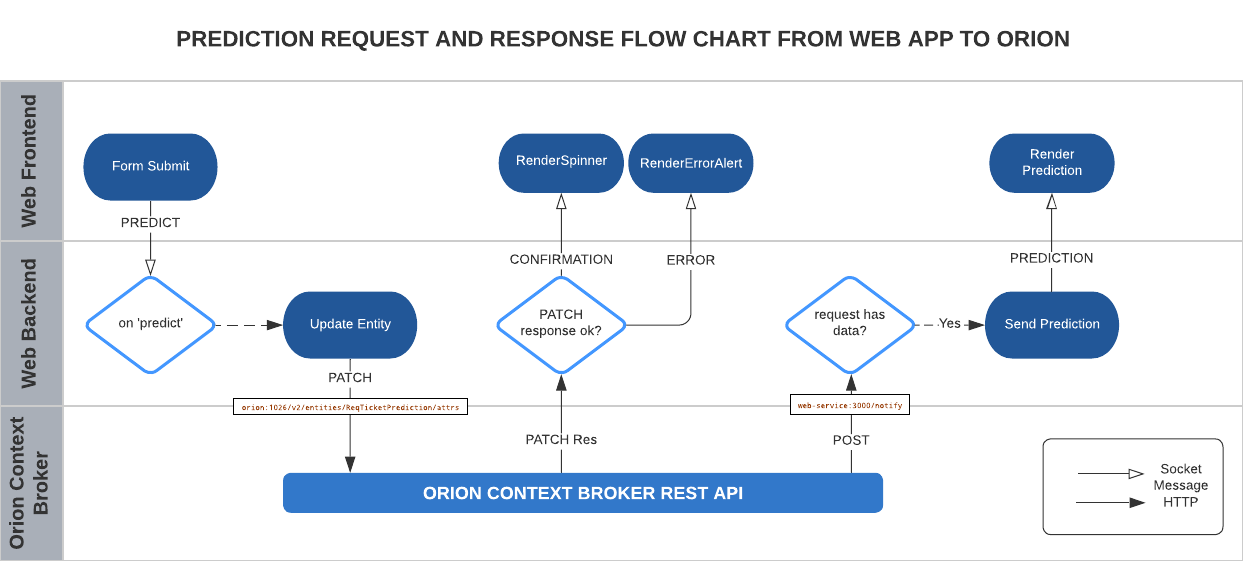
\includegraphics[width=0.9\linewidth]{imagenes/flow-chart-web-orion.png}
	\caption{Prediction request and response flow chart from webapp to orion.}
	\label{flow-chart-web-orion}
\end{figure}

\subsection{Containerization and deployment in Kubernetes}

To deploy our application to the cluster, we should first create a docker container to wrap it. Our docker image will be built based on the node official image, version 12.18.1. We will also pass some environment variables to the image, specifying the different endpoints of the Kubernetes context that the app will need. 

We will create a Deployment in Kubernetes for this components. With a deployment, we will guarantee that we have always one replica of our container running, and if it fails for some reason, the kubelet service will make sure that the container is deployed again. Also, we will create a LoadBalancer service to expose the port 3000 to our local machine, making use of the minikube's services tool.

\begin{figure}[H]
	\centering
	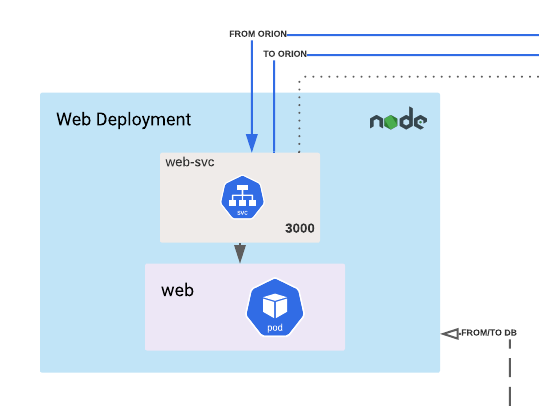
\includegraphics[width=0.5\linewidth]{imagenes/diagram-web-kube.png}
	\caption{Representation of the Kubernetes architecture of the web deployment.}
	\label{diagram-web-kube}
\end{figure}

\clearpage

\section{Database and Data Schemas}
\label{section:DB}

We chose to use MongoDB as our database service for multiple reasons. First and most important, Orion is designed to use MongoDB as the database to store it's context, so we needed it for this purpose. Also, most of the data we are going to work with is already in JSON format, as the NGSI linked data can be serialized to JSON-LD by default. Finally, both Javascript applications and Spark are prepare to easily work with JSON data. So having a central database for all this services was the best option.

As we want our database to be reliable and scalable too, we opted to deploy mongod in replica set mode and as a Kubernetes StatefulSet.

\begin{itemize}
  \item A \textbf{Replica-set} in MongoDB is a cluster of servers that implements replication and automated failover. With this deployment architecture, we will have multiple mongod processes in different Pods managing the same database, and because of this, we will acquire redundancy and a better data availability.
  \item A \textbf{StatefulSet} is the object defined by Kubernetes to manage the deployment of stateful applications, that means, applications with multiple replicas of the same pod that need some guarantees about the order and the state of the running pods. Is the recomended object when deploying databases in cluster mode. (\ref{MongoKubernetes})
\end{itemize}

\begin{figure}[H]
	\centering
	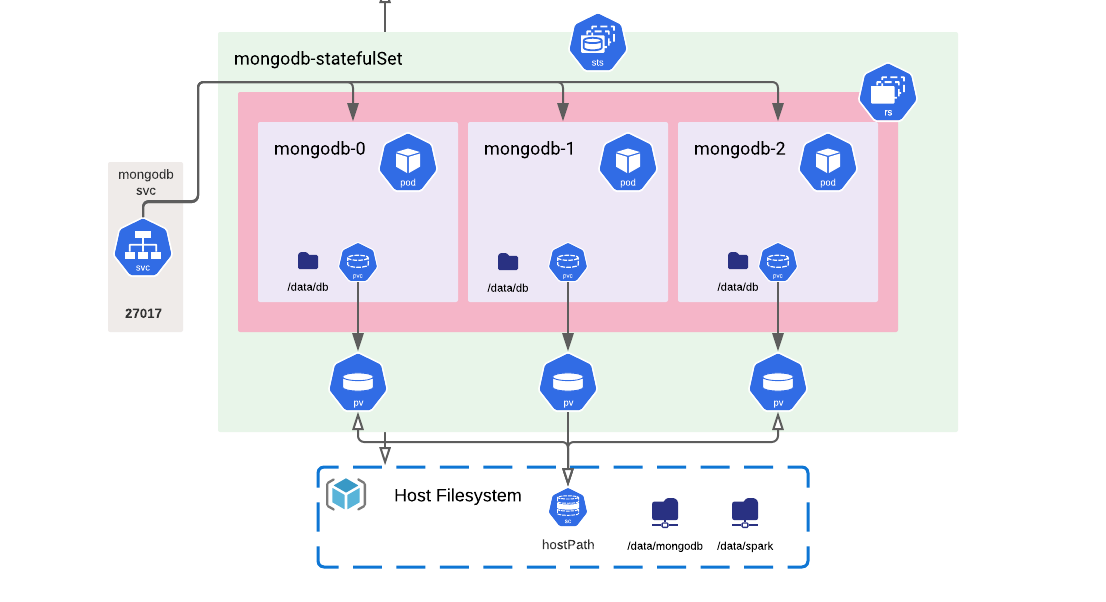
\includegraphics[width=1\linewidth]{imagenes/diagram-db.png}
	\caption{Diagram of the Kubernetes architecture for the database.}
	\label{diagram-db}
\end{figure}

We will also create a PersistentVolume resource, using our hostPath directory as mount point. This will allow us to save the data in a directory of the host where Minikube is running, so we won't loose the data when the cluster goes down. A PersistentVolumeClaim is also needed to map this PersistentVolume with each of the Pods running the mongod process.

Our respective services using the replicaset will automatically create three different databases:

\begin{itemize}
  \item \textbf{Orion}: Created by orion to store information relative to it's entities, subscriptions and internal configuration.
  \item \textbf{Tfm}: We will use this database to save the raw data gathered from the Open Data Platform. This data will be used later to train our model. Another collections with testing purposes will be also created here.
  \item \textbf{Sth\_test}: This database will be created by Draco, to save the list of past predictions requested by the web application. 
\end{itemize}

\clearpage

\section{Fiware: Orion and Draco}
\label{section:Fiware}

The FIWARE components will act as the backbone of our system, providing us with tools to manage our information context and communicate the different services.

The \textbf{Orion Context Broker} will be the main component of our deployment and will administer the context information and data in a decentralized and scalable manner. Orion implements the  FIWARE NGSIv2 API to manage the context information. With this restful API  NGSI, we will be able to perform updates, queries, and change subscriptions on our entities, and also asynchronously connect most of our microservices.

On the other side, we will also use \textbf{Draco}, a FIWARE tool based on Apache NIFI that will power up some of our dataflows. Draco will allow us to create a data pipeline from Orion to our database, so the predictions that go through the Context Broker will be processed and stored in an asynchronous way, so the webapp is able to request them in the future.


\subsection{Orion entities}

In Orion, entities describe the data structure of an object that could be processed by the broker, using the NGSIv2 specification. For example, the temperature of a room could be an entity. 

For our requirements in this project, we only need two different entities. These entities will describe to Orion the kind of objects that can be sent to the broker and their structure. For each attribute of the entity, we will define a name, a value, and a type, which are already defined in the NGSIv2 specification and will help us standardize our data with other context producers and consumers. In this case, we have these two entities:

\textbf{ReqTicketPrediction}:

Defines the input data for our prediction request data flow. The values are set to 0 by default, as we will update this entity with new information every time a user performs a new prediction on the webapp. (\ref{ReqTicketPrediction})

\textbf{ResTicketPrediction}:

Defines the output data for our prediction request data flow. This entity will be updated by the Spark Streaming app, every time a new value is predicted for an input request. (\ref{ResTicketPrediction})


\subsection{Orion subscriptions}

Subscriptions are the mechanism used by Orion to generate a reactive response based on changes in the context information defined by the entities. In our case, we will need to define subscriptions for the predictions requests and responses, and we will also define an additional subscription for Draco.

In Orion, subscriptions are linked to an entity and triggered under the change of certain conditions (i.e. an update of an attribute). Once a subscription is triggered, it will send the specified attributes over the specified notification channel. In our project, this will be an HTTP POST request to the URL of another component of our system. This way, we can asynchronously communicate the components in our data flow using FIWARE standards and controlling the triggering parameters. The defined subscriptions are:

\textbf{subscribeReqPredictionTicket}:

Defines the input data for our prediction request data flow. The values are set to 0 by default, as we will update this entity with new information every time a user performs a new prediction on the webapp. (\ref{subscribeReqPredictionTicket})

\textbf{subscribeResPredictionTicket}:

Defines the output data for our prediction request data flow. This entity will be updated by the Spark Streaming app, every time a new value is predicted for an input request. (\ref{subscribeResPredictionTicket})

\textbf{subscribeResDracoPredictionTicket}:

Defines the subscription that will trigger Draco for post-processing of our prediction. (\ref{subscribeResDracoPredictionTicket})


\subsection{Containerization and deployment in Kubernetes.}

FIWARE provides official and frequently updated docker images for most of their components, and as our project doesn't require any additional configuration to the standart Orion and Draco tools, we will stick to them instead of building our own.

Focusing on Kubernetes configuration, we will define a Deployment to maintain and scale on demand the Orion Pod. As arguments for the configuration of the Orion container, we will specify the database URI and the replica set information, with some additional parameters for improving the performance. The port used for the container will be the default for Orion, 1026. (\ref{OrionKubernetes})

Regarding the Service, we will configure a NodePort service using port 1026 as container port and port 30329 as the external port, as we will need to make HTTP requests from outside of the cluster to configure the entities and subscriptions. (\ref{OrionKubernetesService})

For Draco, Kubernetes configuration will be similar. We will also define a Deployment, with no previous configuration, and, in this case, a normal service exposing both data (5050) and UI (8080) ports. We will use the label service:draco for the match between both components. (\ref{DracoKubernetes} and \ref{DracoKubernetesService})

\subsection{Data flow on Fiware components}

Once we have our components deployed in the cluster, the first step is to configure the Orion entities and subscriptions (just on a fresh start of the containers). We will do that through the NGSIv2 API, doing POST requests from our shell to the configured NodePorts.

To automate this process, we have created a shell script that has all the data already pre-configured. As we are working with Minikube for this example, we only have one node, and we can obtain its IP address by using the *minikube ip* command. Then, we will sequentially call the different scripts. These scripts perform a curl POST command including the object's description in an NGSIv2-compatible JSON format as payload (the JSON we described in the previous section).

\begin{lstlisting}[language=bash,caption=Script to perform the configuration of Orion entities and Subscriptions]
CLUSTER_IP=$(minikube ip)
sh createPredictionEntities.sh $CLUSTER_IP:30329
sh subscribeReqPredictionTicket.sh $CLUSTER_IP:30329
sh subscribeResPredictionTicket.sh $CLUSTER_IP:30329
sh subscribeResDracoPredictionTicket.sh $CLUSTER_IP:30329
\end{lstlisting}

The commands will return a *201 Created* code if everything went ok.

Regarding the database, the configuration is done on the Pod definition template, as we are passing down the parameters to connect to MongoDB. If the connection is successful, Orion will create a new database named Orion, where different collections dedicated to entities, subscriptions, registrations, and internal configurations will be generated.

Once everything is configured, our Context Broker will be ready to interact with other components of our cluster. As we explained, we will update the entities by doing a PATCH request to the API, and if the trigger conditions are met, a notification will be sent to the URL specified in the subscription configuration.

Now, we can improve the flow chart defined in the webapp section by adding Orion to the equation. In the following chart, the interactions between Orion and the surrounding components are explained for the prediction request flow.

\begin{figure}[H]
	\centering
	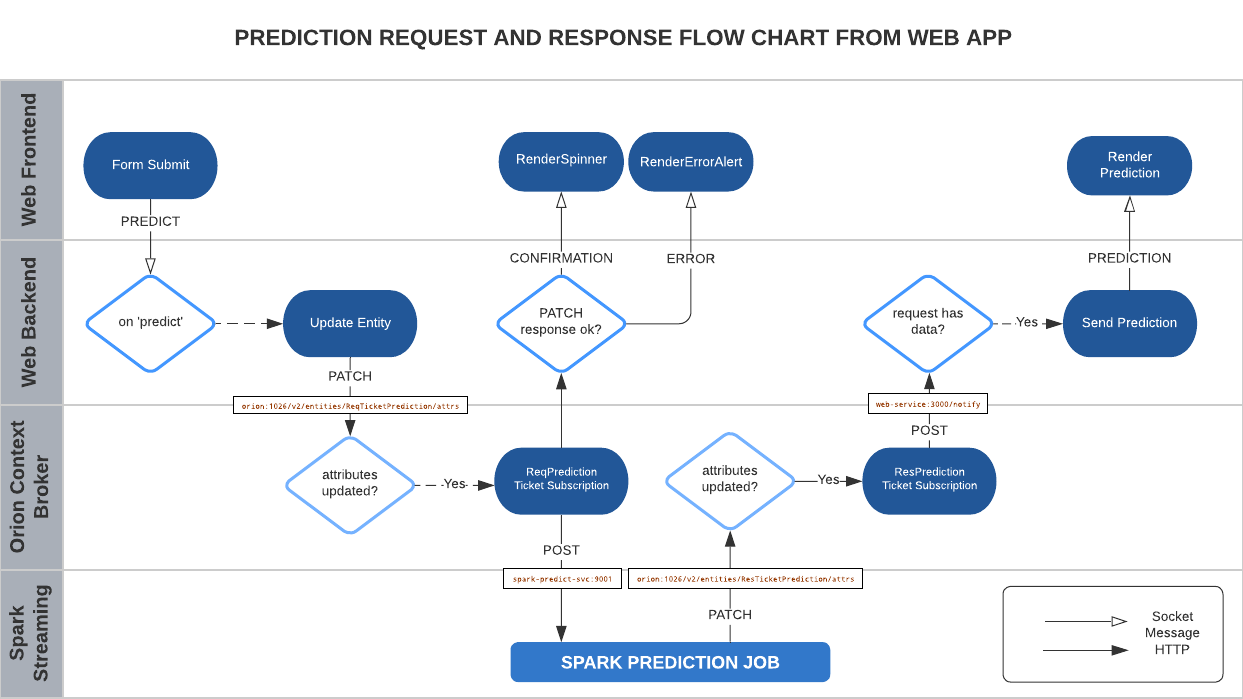
\includegraphics[width=1\linewidth]{imagenes/flow-chart-web-spark.png}
	\caption{Prediction request and response flow chart from webapp to spark.}
	\label{flow-chart-web-spark}
\end{figure}

\subsection{Adding and Configuring Draco}

In the final stages of the development of this proof of concept, we introduced Draco as a tool to help us deal with the processing and storage of the predicted value. Draco is powerful in connecting the FIWARE environment with external tools like databases, acting as a sink where Orion can place the objects to store them, and Draco, thanks to the underlying Apache NIFI, will process them at his own pace.

Also, we can take advantage of the NIFI UI to configure the data flows. Accessing Draco user interface on the service generated by minikube, we can configure the data pipeline that will process our data. Draco will preload some Templates for Nifi, so we can go one from the ORION-TO-MONGO one. This will load a sink pipeline with a HTTP listener module, a module to convert data in NGSI format to JSON and save the input in a collection, and a Logger to keep track of the statistics.

\begin{figure}[H]
	\centering
	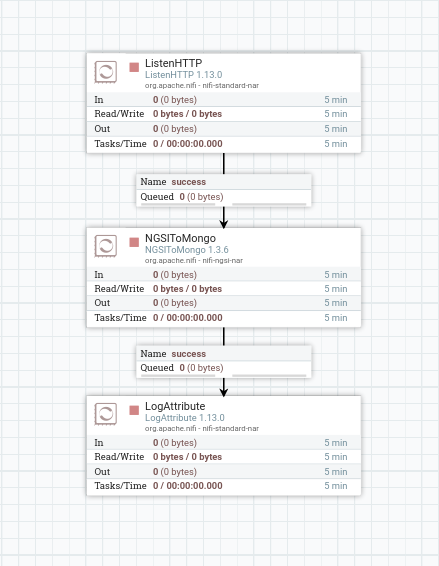
\includegraphics[width=0.7\linewidth]{imagenes/draco-data-routing.png}
	\caption{Graph on Draco UI defining our data routing template}
	\label{draco-data-routing}
\end{figure}

The next step to finish the configuration of Draco will be to edit the parameters of the NGSIToMongo module, so it can properly connect to our database. There, we will configure values like our Replicaset URI, authentication, and the name of the collection.

Once this is done, we can start the Pipeline and Draco will start receiving notifications from Orion once new predicted values arrive. In the following chart, we can see the previous flow updated to include Draco.

\begin{figure}[H]
	\centering
	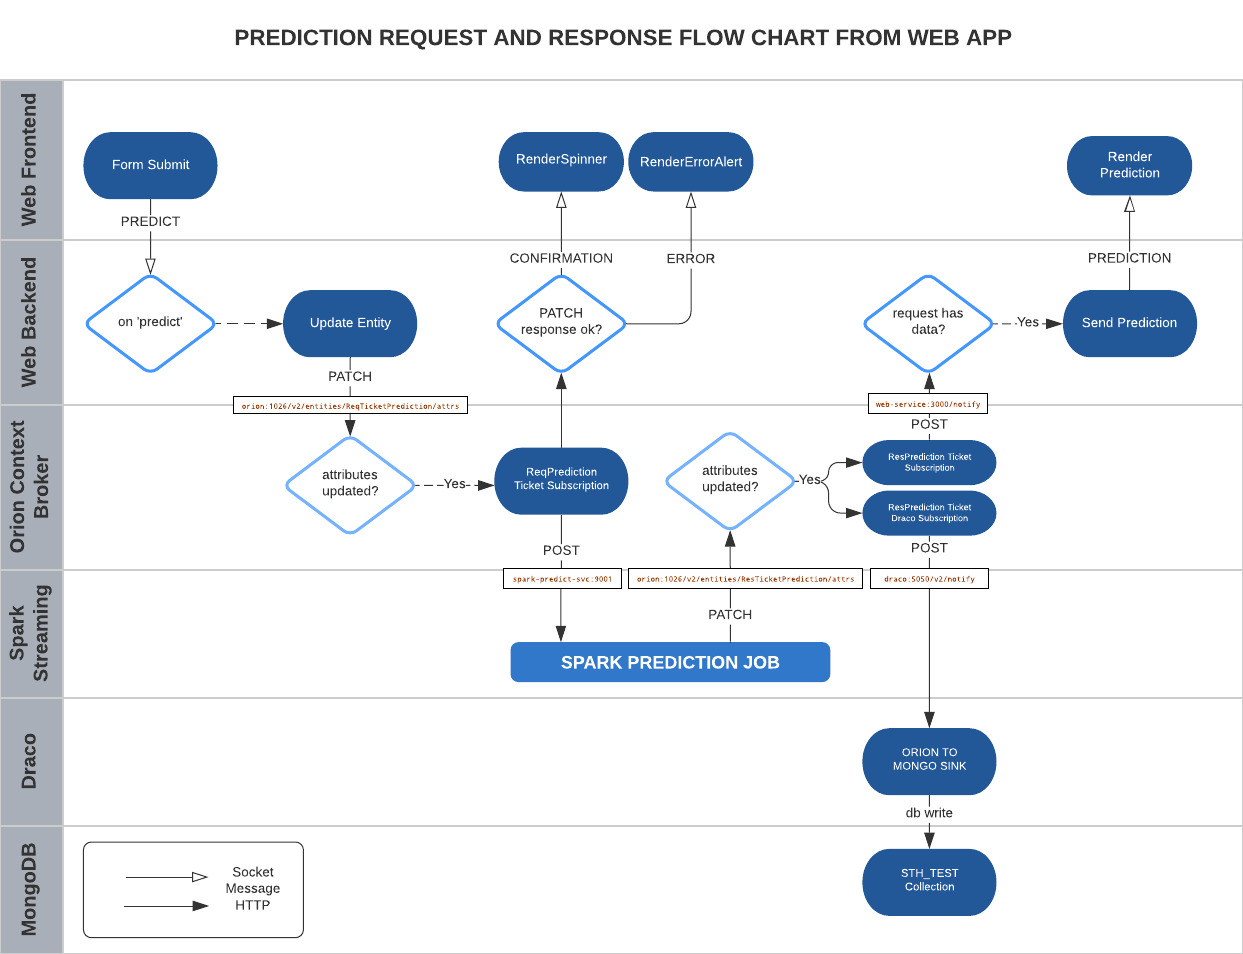
\includegraphics[width=1\linewidth]{imagenes/flow-chart-web-draco.png}
	\caption{Prediction request and response flow chart from webapp to draco.}
	\label{flow-chart-web-draco}
\end{figure}

\clearpage

\section{Machine Learning Model}
\label{section:ML}

In this section, we will discuss the data collection, analysis, and processing stages, as well as the model selection and training, both in Python and in Scala. 

As we discussed in the introduction of this chapter, the data is exposed by a public entity that belongs to the Málaga town hall, SMASSA \cite{smassa}. They are in charge of managing and solving the problems of the public parking of the city, and they are linked to the city Open Data portal, where public data from different sources is exposed so everybody can work with them and collaborate in creating a better and smarter city.

In the Open Data Portal of the Málaga town hall\cite{OpenDataParkingMalaga} , we can find an endpoint where data regarding the parking available spots is published, and this will be our main data source. Unfortunately, they do not have available yet a dataset with past data, and they only publish a new JSON or CSV document every minute with the real-time values for all the Parkings of the city, so we had to come up with a solution to have a dataset to train our model. 

We will go in deep on this solution in the next section, so for now let's suppose that all the data is already in our MongoDB database as raw data in the NGSIv2 JSON format.

\subsection{Our source data}

Our system has collected data since it started working, on July 27th of 2021, and besides some corrupted data on a couple of weeks in September, it has been working until the end of the year. This may seem as not enough data to feed a sufficiently good machine learning algorithm, but the results so far are acceptable, and the idea is that if we maintain this system running in the future, it will automatically fetch new data each minute, and train the model every month adding the new information to the dataset, so the model will improve over time. 

There is available data for ten public parking facilities around the city, and as the data is gathered every minute, we have almost 3.000.000 values in total on the day this document is written. The availability data is exposed in the FIWARE NGSI format, where a lot of context information about the location and facility where the value was produced is added, with the idea of allowing different types of integrations. Here, you can see an example of a value fetched from the portal: 

\begin{lstlisting}[language=json, caption=Example of a NGSI JSON object fetched from the Málaga Town Hall Open Data Portal.]
{ 
    "name": {
        "type": "Text", 
        "value": "Salitre"
    }, 
    "availableSpotNumber": {
        "type": "Integer", 
        "value": "168", 
        "metadata": {
            "timestamp": {
                "type": "DateTime", 
                "value": "None"
            }
        }
    }, 
    "source": {
        "type": "Text", 
        "value": "https://datosabiertos.malaga.eu/recursos/aparcamientos/ocupappublicosmun/ocupappublicosmunfiware.json"
    }, 
    "totalSpotNumber": {
        "type": "Integer", 
        "value": -1
    }, 
    "location": {
        "type": "geo:json", 
        "value": {
            "type": "Point", 
            "coordinates": ["-4.4276681", "36.7132149"]
        }
    },  
    "owner": {
        "type": "Text", 
        "value": "https://www.smassa.eu/"
    }, 
    "occupancyDetectionType": {
        "type": "Array", 
        "value": ["singleSpaceDetection"]
    }, 
    "dataProvider": {
        "type": "Text", 
        "value": "https://www.smassa.eu"
    }, 
    "type": "OffStreetParking", 
    "id": "Salitre", 
    "description": {
        "type": "Text", 
        "value": "Calle SalitreM\u00e1laga"
    }
}
\end{lstlisting}

Some of the values have been suppressed, as they were not relevant for our example. Here, we can see the Parking name and the number of available spots at that time, along with other values as the location of the facility, the type of parking, or the type of detection used for doing the calculation. 

All the data is described using an Open Data format, where each value has a type field describing the Context of the value. As you can see, the Date and time information is not included in the provided data, but we have solved this by editing the DateTime value in the metadata field at the time of the data harvesting. We will describe this modification in the next section. The data regarding the total number of available spots for parking in each facility was also missing, but we found this data in the SMASSA webpage, and we have created an object to use these values in the data transformation stage. 

The interesting values for us are the Parking ID, the date and time the value was generated, and the available spot number for this combination. Starting from here, we deployed a Jupyter notebook in our Kubernetes cluster to analyze and test the data. This makes it easier to understand how are the values distributed across time, and test which machine learning classification model fits better our needs. 

\clearpage

\subsection{Data transformation and analysis}

For the data analysis and inspection, we loaded all the values from October and November to the notebook, using the \textit{pymongo}\cite{pymongo} library to connect to the database service and fetch the documents. We only want to keep some of the values that actually form the object, so we will create a new pandas DataFrame with these values, and start the data processing. The steps we followed to prepare and transform the data, as a brief summary are:

\begin{itemize}
    \item Extract the data from the raw JSON object and create a new dataframe, containing the Parking ID, the DateTime string, and the number of available spots.
    \item Transform the Parking name so it doesn’t include any exceptional character that could be wrongly processed by the algorithm, as accents or whitespaces.
    \item Convert the date and time string to a proper DateTime object, which will be converted to date and time-related values in the following steps.
    \item Convert the number of available spots in an Integer, and drop the not available values from the DataFrame. Not available values are defined as a -1 if they were generated by the source, and a None value if they were corrupt or wrongly processed at the fetching time. We should handle both cases.
    \item We will add the total number of spots for each facility from a statically-generated list.
    \item We will calculate the occupation of the facility for each value dividing the available spots by the total number of spots in the facility, and then rounding it and inverting the value. This will result in a percentage of the occupation, in intervals of 10%.
    \item From the datetime object, we will extract interesting data for our model, as the day of the week, the day, the hour, or the month when the value was generated.
\end{itemize}

After this first pre-processing, we inspected the data to search for patterns and interesting correlations between input data. This is the head of our DataFrame at this point of the analysis (Figure \ref{dataframe-no-preprocessing}):

\begin{figure}[H]
	\centering
	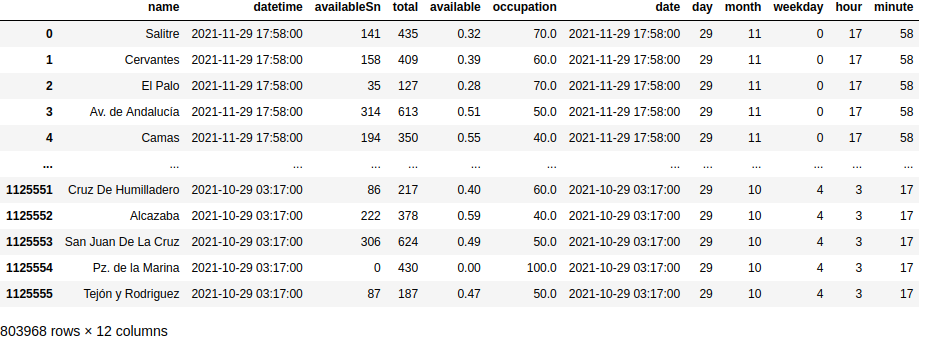
\includegraphics[width=1\linewidth]{imagenes/dataframe-no-processing.png}
	\caption{Dataframe after data preprocessing. Some interesting insights were extracted from the original values.}
	\label{dataframe-no-preprocessing}
\end{figure}

Now we can represent this data to search patterns. First, we represented the occupation level for each parking facility in intervals of 4 hours, and we can plot it as a line plot (Figure \ref{parking-occupation-time}). This is not the cleanest way of visualizing the data, but it can help to visualize the occupation of each parking independently through time.

\begin{figure}[H]
	\centering
	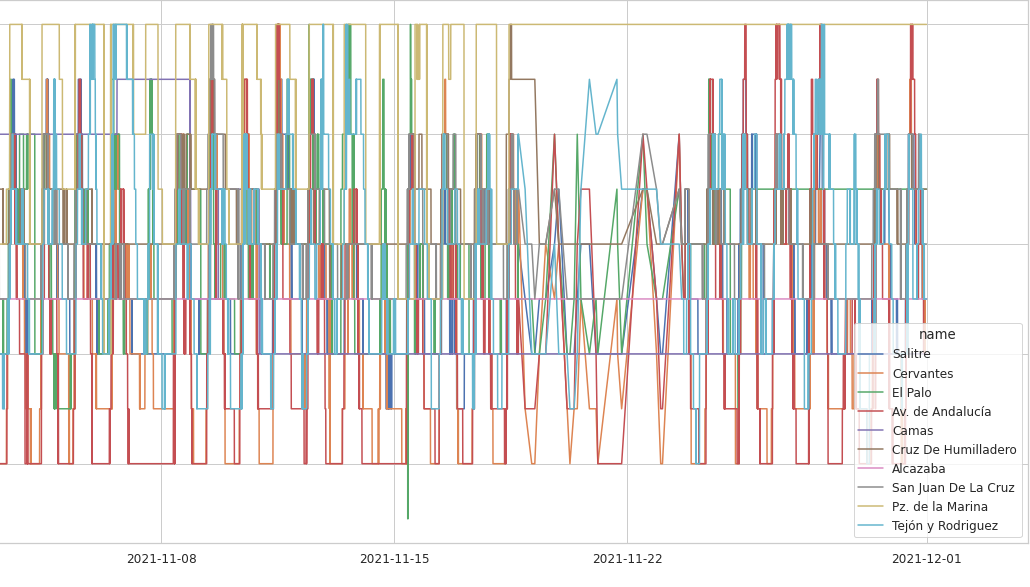
\includegraphics[width=1\linewidth]{imagenes/parking-occupation-time.png}
	\caption{Parkings occupation through time (October and November).}
	\label{parking-occupation-time}
\end{figure}

For a cleaner visualization, we can do the same but aggregating the values by the mean of all the facilities for a certain time interval (Figure \ref{parking-mean-occupation-time}). Here, we can start to see some patterns, depending on the time of the day and the day of the week. We can easily detect the bigger affluence on the weekends, as well as the increase of the occupation in the holidays.

\begin{figure}[H]
	\centering
	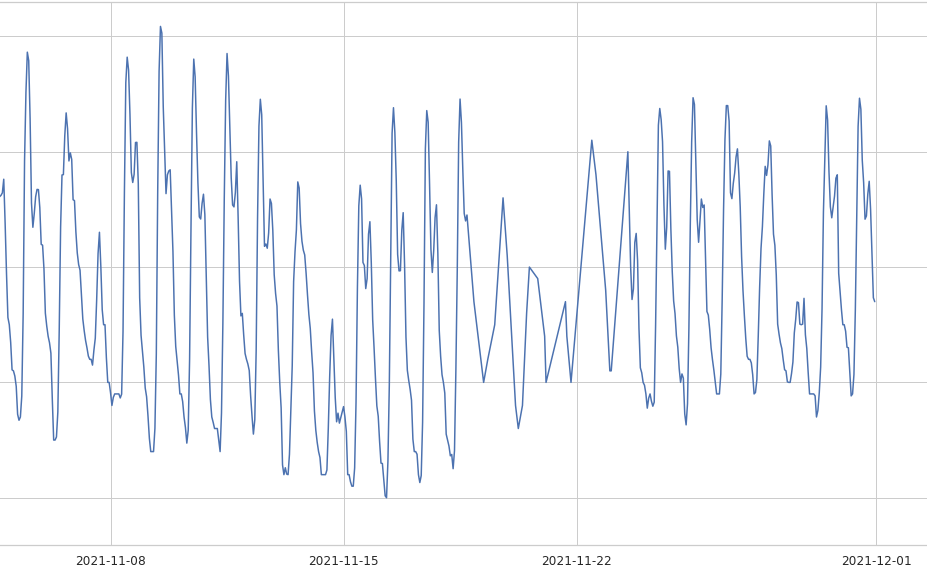
\includegraphics[width=1\linewidth]{imagenes/parking-mean-occupation-time.png}
	\caption{Parkings occupation through time (October and November).}
	\label{parking-mean-occupation-time}
\end{figure}

Focusing on these patterns, we can further explore them by aggregating the data for each feature. We can, for example, plot the mean occupancy for each day of the week, or by the time of the day. This way, we obtain these really interesting graphs.

In this first plot, we can see how the day of the week is somehow important for the occupation level, but it depends on the parking facility. Also, we can extract that depending on the parking, the occupation will increase on the weekends, or decrease, probably based on its location. Parking lots close to work areas outside of the city center will have lower affluence on the weekends, while those in the city center will tend to be more crowded.

\begin{figure}[H]
	\centering
	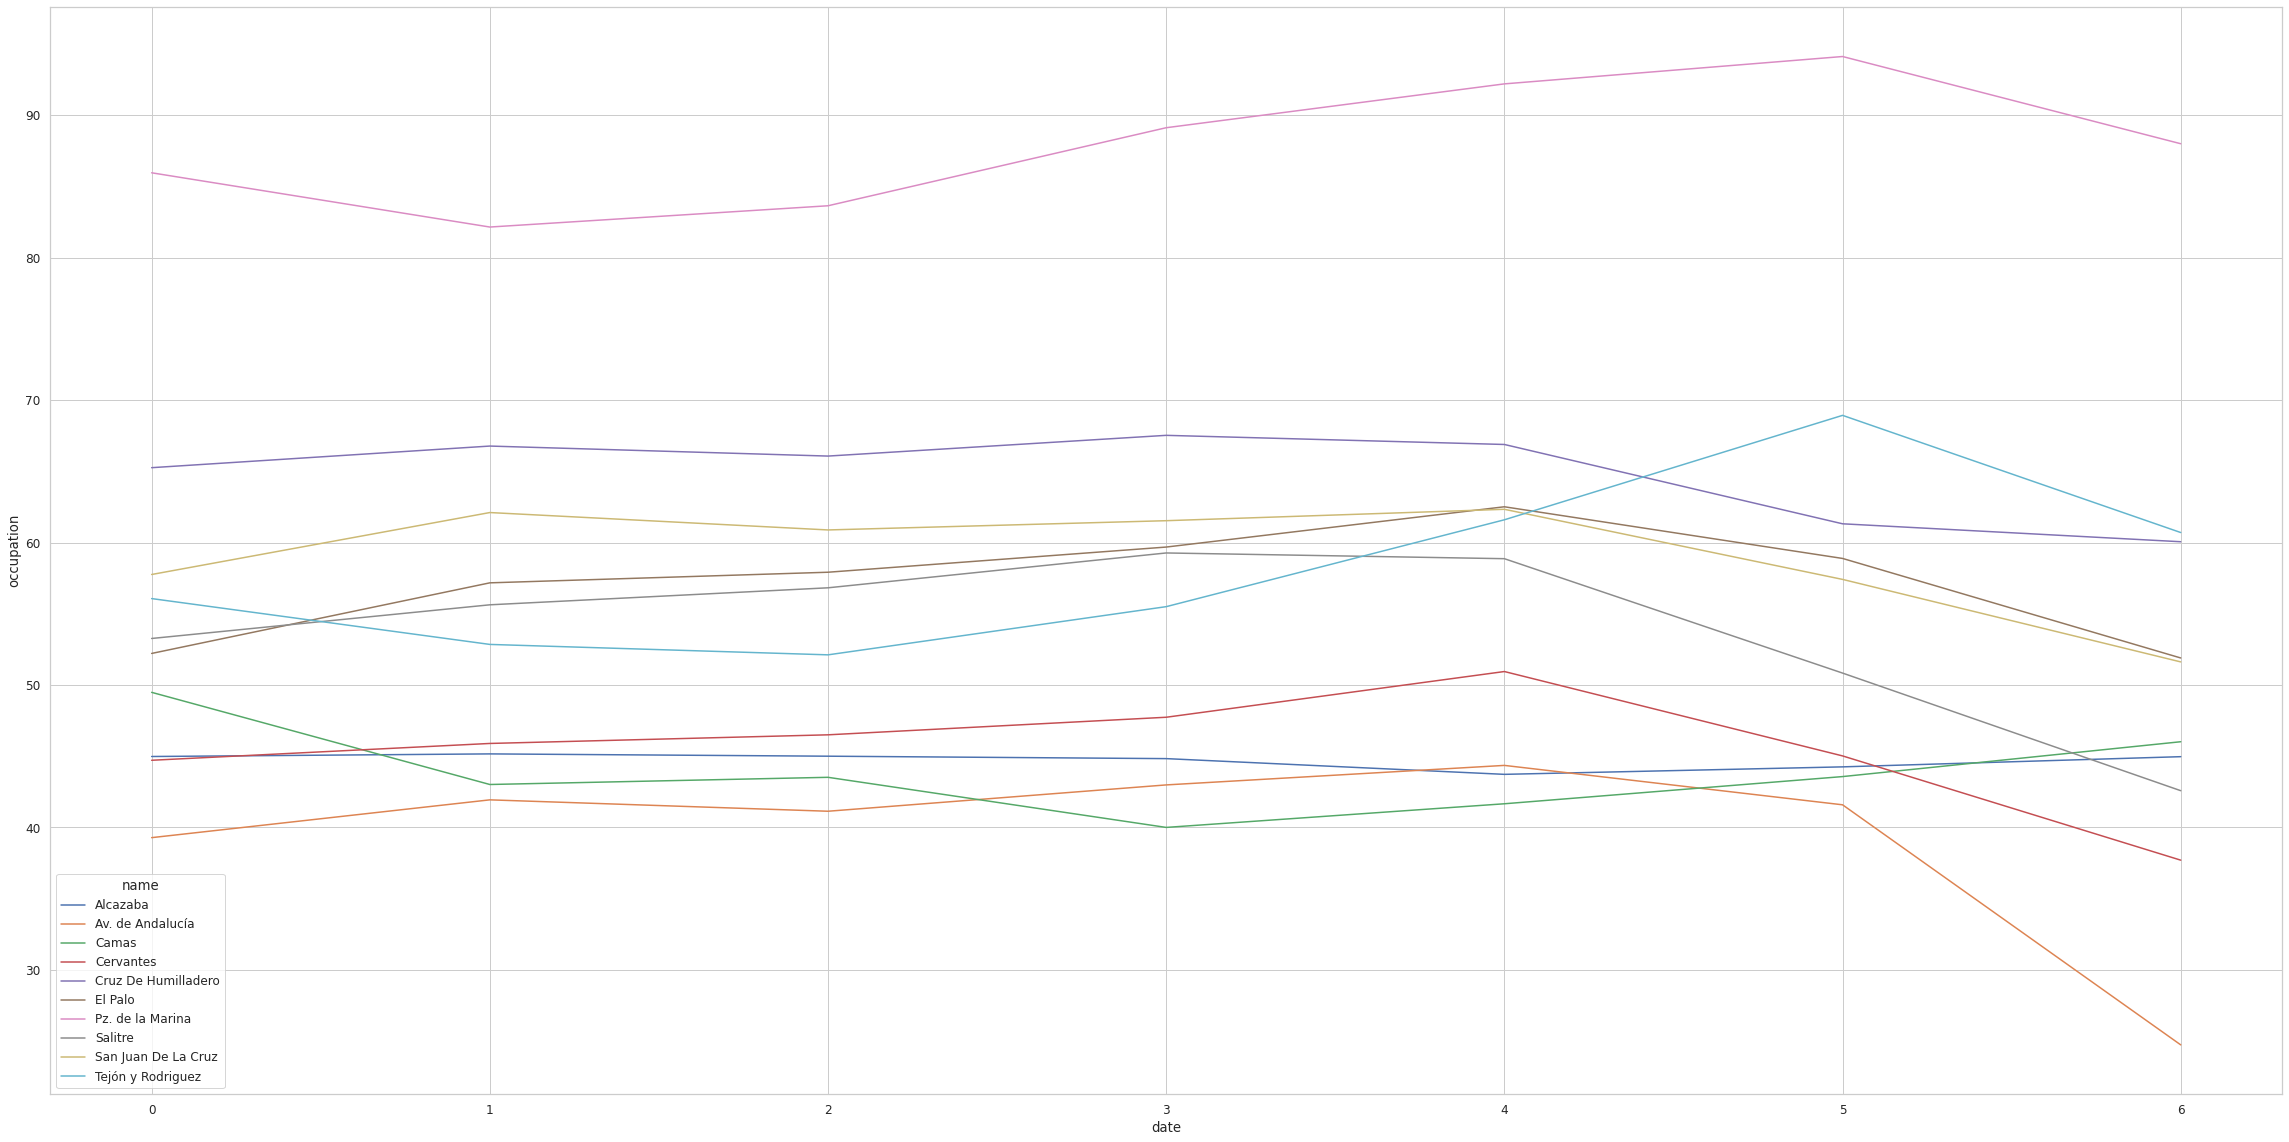
\includegraphics[width=0.9\linewidth]{imagenes/aggregated-mean-occupation-week.png}
	\caption{Aggregated mean parking occupation depending on the day of the week (0-Monday, 6-Sunday).}
	\label{aggregated-mean-occupation-week}
\end{figure}

On the other hand, if we look at the aggregated occupation depending on the hour of the day, we could see a strong correlation for most of them, decreasing the occupation during the night and with a strong increase in the morning.

\begin{figure}[H]
	\centering
	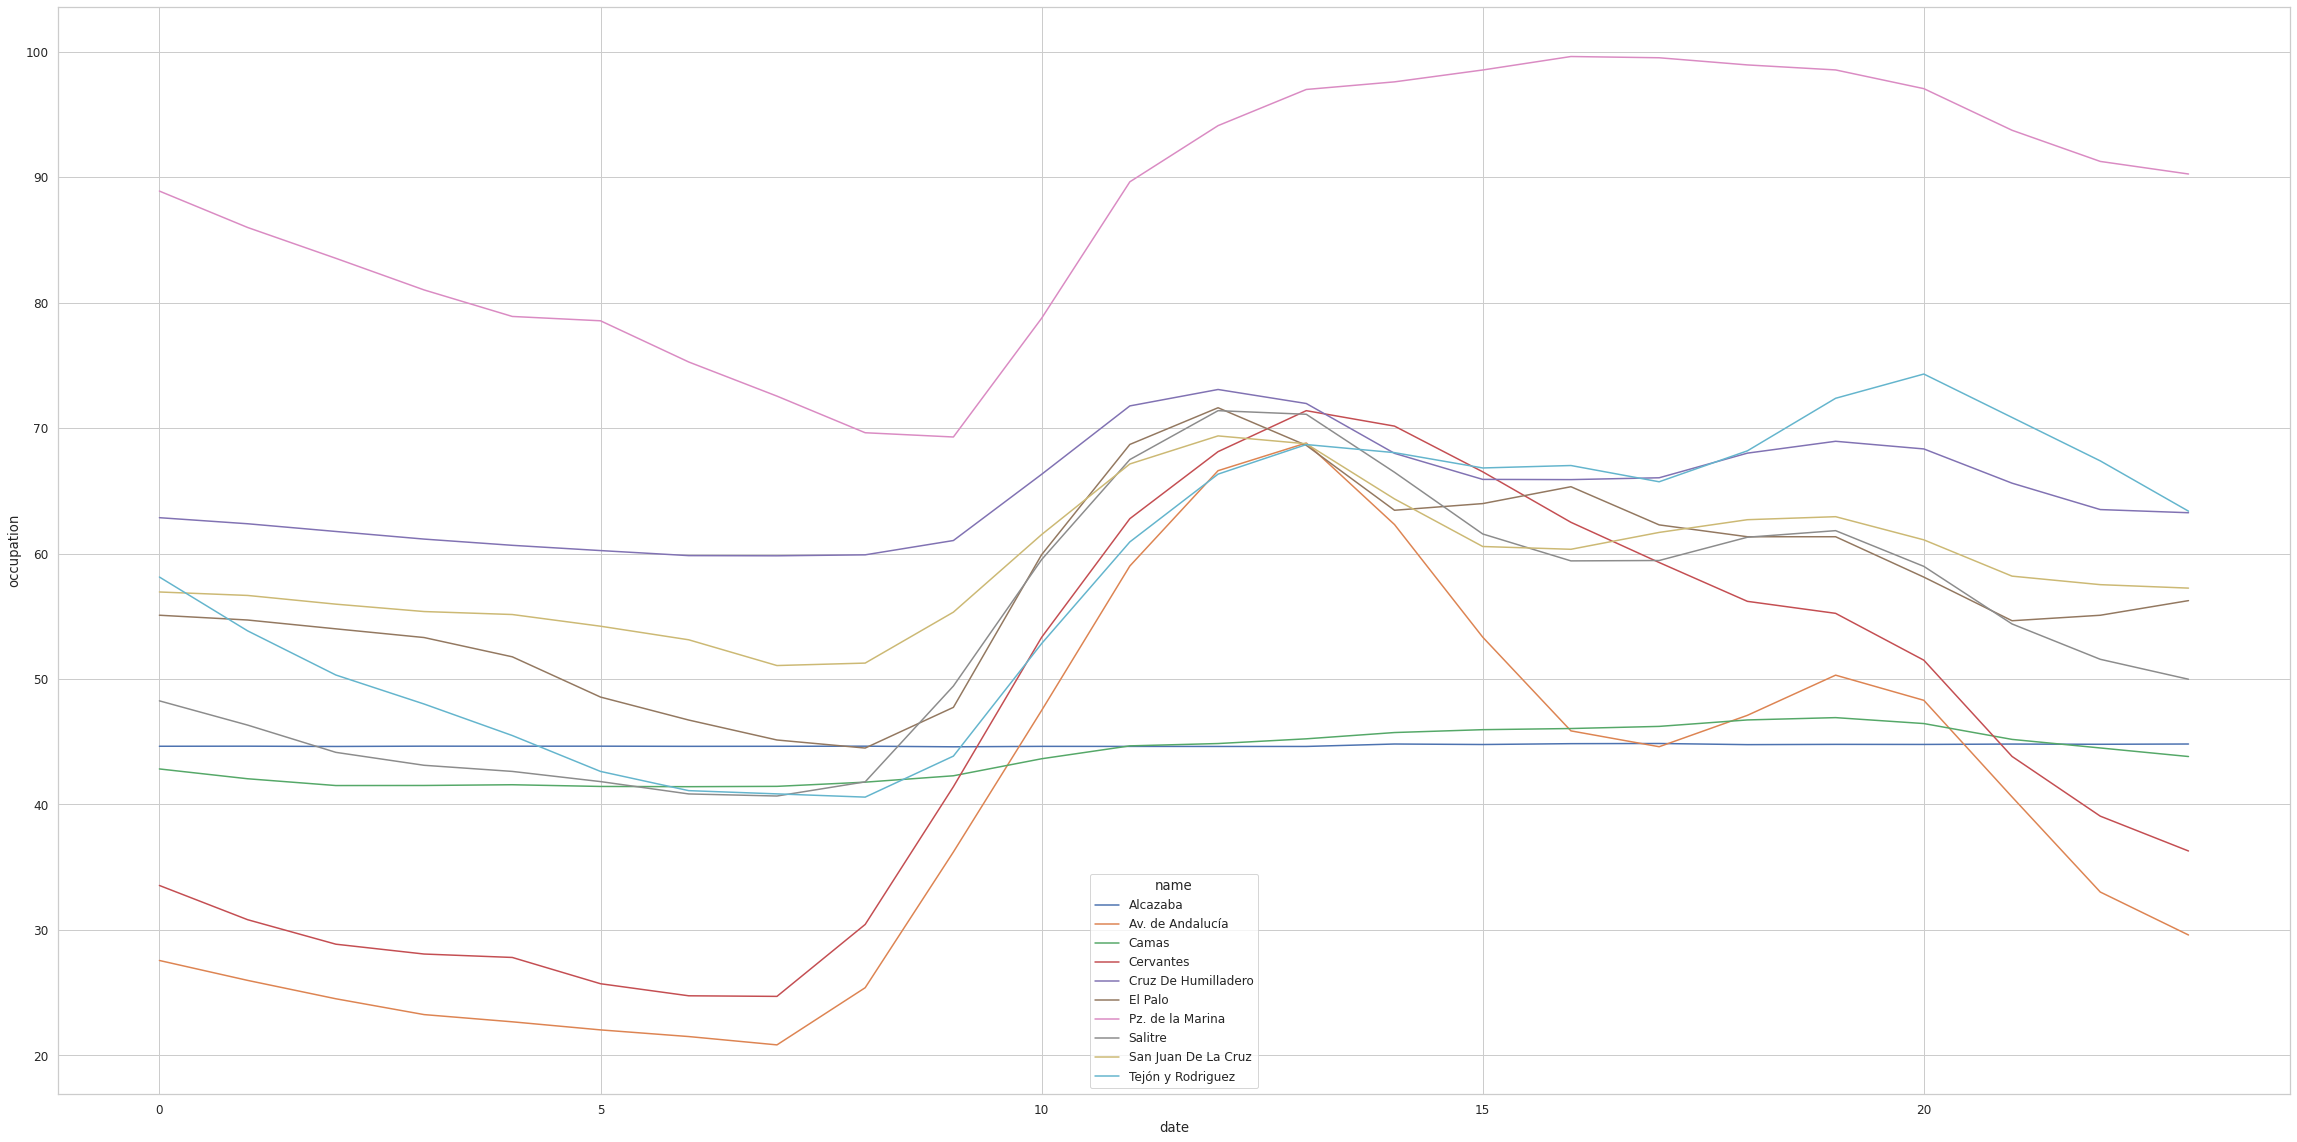
\includegraphics[width=0.9\linewidth]{imagenes/aggregated-mean-occupation-hour.png}
	\caption{Aggregated mean parking occupation depending on the hour of the day.}
	\label{aggregated-mean-occupation-hour}
\end{figure}

Also in this graph, we noticed that the values for the facilities of Alcazaba and Camas are almost continuous, and after a deeper look into the data, we found that the values for Alcazaba were odd, having its occupation around 45 percent for the whole period when data was been collected. This forced us to discard this facility for the moment, until we have better data.

\clearpage

\subsection{Model selection}

After processing the data, our next step is to select the best features and compare training results on different models. We did this on our Jupyter Notebook, and in the following sections we will move our model to Scala in order to integrate it with our system.

Due to the lack of data from previous years, it doesn't seem like the feature year will have any weight in the predictions, so we discarded it for now. Taking this into account, we have five features to work with: The facility name, which we will index in order to pass it to the model, and the time variables like the hour, day, weekday (also indexed from 0-Monday to 6-Sunday), and the month. These are the different available features.

\begin{table}[H]
    \begin{tabular}{|c|c|c|c|c|c|c|}
    \hline
    \textbf{Feature} & name            & hour         & weekday      & day          & month        & \begin{tabular}[c]{@{}c@{}}occupation\\ (label)\end{tabular} \\ \hline
    \textbf{Type}   & \textit{String} & \textit{Int} & \textit{Int} & \textit{Int} & \textit{Int} & \textit{Int}                                                 \\ \hline
    \textbf{Values}       &  "Name"   & {[}1-24{]}   & {[}0-6{]}    & {[}1-31{]}   & {[}1-12{]}   & {[}0:10:100{]}\%                                             \\ \hline
    \end{tabular}
    \caption{Features name, type and available values.}
\end{table}

There are two different approaches on how to face our model search, as we first have to decide if we can face this problem as a classification or a regression problem. Our variable to predict is given as a continuous value, as the available number of spots in each parking facility for a given time. We could feed this data to a regression model, and try to predict the available number of parking spots comparing it to the existing values and extracting, for example, the RMSE (rooted mean square error) to evaluate the model. The other option is to manipulate the label variable so we can convert our label into a categorical variable, as the percentage of occupation from 0 to 100 percent, in intervals of 10 units. This second approach will simplify the complexity of our model, and increase its accuracy. As we don’t need the exact value of available spots, an estimation of the occupation of the facility seems like an easier and more precise model, so we will proceed with this solution.

We will select six classification models, and we will compare all of them setting up a cross-validation function that will provide us a more reliable evaluation of each individual model, so we can have a better overview of which models work better for our data. We will do this process several times, changing the provided set of features so we can compare how different combinations perform.

The models we will tests are:
\begin{itemize}
    \item \textbf{LogR}: Logaritmic Reggresor
    \item \textbf{LDA}: Linear Discrimination Analysis
    \item \textbf{KNN}: K-nearest Neighbors
    \item \textbf{DTC}: Decision Tree Classifier
    \item \textbf{RFC}: Random Forest Classifier
    \item \textbf{SGD}: Stochastic Gradient Descent Classifier
\end{itemize}

And the acronyms used for the feature variations are:
\begin{itemize}
    \item \textbf{NM}: Month feature not included
    \item \textbf{M}: Month feature included
    \item \textbf{NI}: Name feature indexed
    \item \textbf{NC}: Name feature codified
    \item \textbf{WC}: Week feature codified
\end{itemize}

\begin{table}[H]
    \begin{tabular}{|l|l|l|l|l|l|l|}
    \hline
    \textbf{Ft}                                                  & \textbf{LogR}                                        & \textbf{LDA}                                                  & \textbf{KNN}                                                  & \textbf{DCT}                                              & \textbf{RF}                                                   & \textbf{SGD}                                                 \\ \hline
    \textit{\begin{tabular}[c]{@{}l@{}}NI \\ NM\end{tabular}}    & \begin{tabular}[c]{@{}l@{}}0.44423\\ (0.00196)\end{tabular} & \begin{tabular}[c]{@{}l@{}}0.42004\\ (0.001)\end{tabular} & \begin{tabular}[c]{@{}l@{}}0.54821\\ (0.00227)\end{tabular} & \begin{tabular}[c]{@{}l@{}}0.58465\\ (0.00181)\end{tabular} & \begin{tabular}[c]{@{}l@{}}0.58483\\ (0.00192)\end{tabular} & NA                                                           \\ \hline
    \textit{\begin{tabular}[c]{@{}l@{}}NI\\ M\end{tabular}}      & \begin{tabular}[c]{@{}l@{}}0.44423\\ (0.00196)\end{tabular} & \begin{tabular}[c]{@{}l@{}}0.42023\\ (0.00184)\end{tabular} & \begin{tabular}[c]{@{}l@{}}0.54212\\ (0.00204)\end{tabular} & \begin{tabular}[c]{@{}l@{}}0.59463\\ (0.00136)\end{tabular} & \begin{tabular}[c]{@{}l@{}}0.59502\\ (0.00127)\end{tabular} & \begin{tabular}[c]{@{}l@{}}0.38345\\ (0.00593)\end{tabular} \\ \hline
    \textit{\begin{tabular}[c]{@{}l@{}}NC\\ M\end{tabular}}      & \begin{tabular}[c]{@{}l@{}}0.45317\\ (0.00135)\end{tabular}  & \begin{tabular}[c]{@{}l@{}}0.4216\\ (0.00150)\end{tabular}  & \begin{tabular}[c]{@{}l@{}}0.54927\\ (0.00269)\end{tabular} & \begin{tabular}[c]{@{}l@{}}0.59480\\ (0.00129)\end{tabular} & \begin{tabular}[c]{@{}l@{}}0.59451\\ (0.00166)\end{tabular} & \begin{tabular}[c]{@{}l@{}}0.4012\\ (0.00751)\end{tabular} \\ \hline
    \textit{\begin{tabular}[c]{@{}l@{}}NC\\ WC\\ M\end{tabular}} & \begin{tabular}[c]{@{}l@{}}0.42142\\ (0.00169)\end{tabular}  & \begin{tabular}[c]{@{}l@{}}0.41991\\ (0.00168)\end{tabular} & \begin{tabular}[c]{@{}l@{}}0.54811\\ (0.00254)\end{tabular} & \begin{tabular}[c]{@{}l@{}}0.59648\\ (0.00168)\end{tabular} & \begin{tabular}[c]{@{}l@{}}0.61502\\ (0.00100)\end{tabular} & \begin{tabular}[c]{@{}l@{}}0.41531\\ (0.0102)\end{tabular} \\ \hline
    \end{tabular}
    \caption{Comparaison of cross-validation evaluation results for different classification models and feature combination. Mean accuracy and standart deviation.}
\end{table}

These results were obtained through a k-fold Cross-Validation method. Specifically, we used a 10-fold random validation, so for each model, we performed the training process using one of each 10 splits of the dataset as our test data, and the other 9 as the train data, obtaining an array of evaluations, in this case the accuracy. Then, what is displayed is the mean accuracy and the standard deviation for the specific model. \\

\begin{lstlisting}[language=Python, caption=Portion of the code we used for the cross-validation of the models]
for name, model in models:
	kfold = model_selection.KFold(n_splits=10, random_state=seed,shuffle=True)
	cv_results = model_selection.cross_val_score(model, X, Y, cv=kfold, scoring='accuracy')
	results.append(cv_results)
	names.append(name)
	msg = "%s: %f (%f)" % (name, cv_results.mean(), cv_results.std())
\end{lstlisting}

As the algorithm that outperformed the others was the Random Forest Classifier, we tried to improve its results by tuning the hyperparameters. In order to search for the best combination of inputs, we performed a GridSearch, that evaluates the model using cross-validation for different parameters, and outputs the combination of values that showed a better result.

We performed this grid search modifying the number of trees, from 200 up to 700, and by changing the max-features parameter of the algorithm. This defines the maximum number of features Random Forest is allowed to try in an individual tree, and there are three available options. Basically, this limits the number of features allowed up to the number of features provided (auto), up to the square root of the number of features (sqrt) or up to the base two logarithm of the number of features (log2). \\

\begin{lstlisting}[language=Python, caption=Portion of the code we used for performing the parameters grid search.]
rfc = RandomForestClassifier(n_jobs=-1,max_features= 'sqrt' ,n_estimators=50, oob_score = True) 
param_grid = { 'n_estimators': [200, 700],'max_features': ['auto', 'sqrt', 'log2']}
CV_rfc = GridSearchCV(estimator=rfc, param_grid=param_grid, cv= 5)
CV_rfc.fit(X, Y)
print(CV_rfc.best_params_)
\end{lstlisting}

With this tuning, we found that the best parameters for this setup were \textit{'max\_features': 'log2', 'n\_estimators': 200}, and after doing a new cross-validation with these parameters, we managed to increase the accuracy up to 0.662830 (0.001354). Doing a deeper analysis of the final model metrics, we obtained the confusion matrix and confidence intervals before moving to Scala.

\begin{figure}[H]
	\centering
	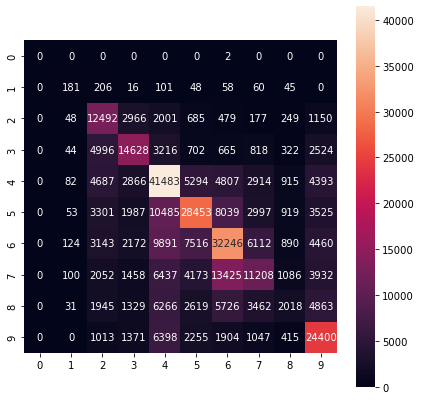
\includegraphics[width=1\linewidth]{imagenes/confusion-matrix.png}
	\caption{Confusion matrix representing our 10 target classes for our final model}
	\label{confusion-matrix}
\end{figure}

As we can see from Figure \ref{confusion-matrix}, even when our accuracy is not really good, the predictions are usually close to the target category, and we have to take into account the fact that our dataset is still limited. This issue should be solved in the future as the dataset grows bigger and consequently, our model has more inputs to learn the problem better.

In the next section, we will move our model to Spark, to deploy it in our Kubernetes cluster and integrate it with our complete workflow.

\clearpage

\section{Spark and Spark Streaming}
\label{section:Spark}
Apache Spark\cite{spark} is an open-source programming framework for distributed data processing designed to be fast and general purpose\cite{spark}. It can quickly perform processing tasks on very large data sets, and can also distribute data processing tasks across multiple computers. These properties fit really good our project needs, so it can be a perfect solution for our data processing stage.

Spark is designed for running Big Data and Machine Learning tasks at scale, as it has been designed from the core to be able to parallelize and break up tasks in smaller pieces, that we can distribute in multiple servers for processing them, and that later can be combined again to get I final result. In our system, we will use Spark for training our models, and later, use those models to make predictions on incoming requests, using Spark Streaming.

We have two options for deploying a Spark application to a cluster, \textbf{Client mode}, and \textbf{Cluster mode}. The main difference is where will the driver application run, and depending on your system requirements and where are you deploying this app, one option will be better than the other. In our case, as our development environment is separated from our cluster, we will opt for the Cluster mode approach.

\begin{figure}[H]
	\centering
	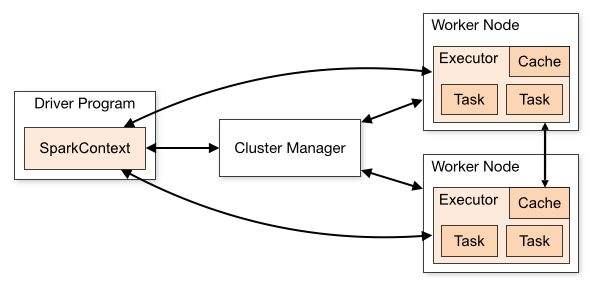
\includegraphics[width=1\linewidth]{imagenes/spark-modes.png}
	\caption{Spark application architecture. From Apache Documentation\cite{spark}.}
	\label{spark-modes}
\end{figure}

As we are deploying our Spark applications to Kubernetes, we have two options depending on our system specifications. Spark adopts a Master/Slave approach whereby a \textit{driver program} (“the master”) creates a \textit{SparkContext} object that connects to a \textit{cluster manager}. This SparkContext is actually an abstraction of the system where it will be executed, and uses it as a unique node where tasks are distributed. The difference then lies in where the cluster manager runs, and even though Kubernetes is supported as a cluster manager since the last Spark update, we stuck to the Standalone cluster manager, where it will run in the node we use for development (outside of the cluster), and will behave as a fire-and-forget process.

Once we submit our Spark application using the spark-submit tool shipped with the spark binaries, it will create a SparkContext (defined in the application code), that will ask the kube-apiserver to set up a driver Pod using a specific image and deploy some executors. Then it will proceed to run the workload on them.

\subsection{Model definition in Spark. Train and Prediction jobs}

In the first iterations of the project, we developed everything with PySpark and MLib, two frameworks for developing Spark applications for machine learning with Python, as we had the advantage of being able to use Jupyter notebooks shipped with Spark to test and debug the code. But after some iterations, we found a lot of issues with the dependencies, and some versions were incompatible with the rest of our Cluster. Also, the Orion connector for Spark was already developed for Scala, and after some failed attempts to adapt it to PySpark, we decided to move all our code to Scala.  

The project will be built using Scala version \textit{2.12.13} and Spark \textit{3.0.1}, so we can be compatible with the MongoDB and the Orion connector libraries. We will use SBT \cite{sbt} as our compiler and build tool, so it has to be properly configured with our build and dependencies requirements. First step is to define our \textit{build.sbt} configuration file to include the required dependencies and our build versions. The idea is to create a fat jar binary that will be shipped with the Docker image to the cluster, and the instructions on how to run the programs will be defined in the SparkContext.

The required additional dependencies that we must include are:
\begin{itemize}
    \item \textbf{Spark MLlibs:} The library for creating and executing machine learning models on Spark\cite{ml-spark}.
    \item \textbf{MongoDB Spark Connector:} With the connector, we will have access to all Spark libraries for use with MongoDB datasets. We will use this connector to fetch the training data from the Parking collection.
    \item \textbf{Orion Spark Connector:} Used for interacting with the Orion NGSI API, receive notifications and send a reply with the results.
\end{itemize}

We will define two main Scala classes, Train and Pedict. The \textbf{Train} object, will trigger a SparkSession that will be in charge of:
\begin{itemize}
    \item Start the Spark Session and pass the Context to the executors.
    \item Connect to the MongoDB and fetch the whole parking dataset.
    \item Convert the raw data from the received RDD to a Dataframe.
    \item Transform the data to obtain the desired features and index and encode the required ones.
    \item Define the RandomForestClassifier model with the expected parameters.
    \item Train the whole Pipeline and the model with the DataFrame.
    \item Evaluate the model and store the results for future comparaison.
    \item Save the model and the processing pipeline in the cluster storage.
    \item End the session.
\end{itemize}

The \textbf{Predict} class, on the other hand, will create a Spark Streaming Session instead of the standart one. As we already explained in the previous chapter \ref{chapter:StateOfArt}, Spark Streaming extends Spark focusing on live data streams processing, providing us with better tools to keep our system listening for new prediction on real time. Predict object, will handle the following tasks:

\begin{itemize}
    \item Start the Spark Streaming Session, and pass the Context to the executors.
    \item Start event streams listen service for notifications on the port 9001.
    \item Receive the prediction notification from Orion, and create a Streaming RDD with the request payload.
    \item Load the model and the processing pipelines from the cluster storage.
    \item Transform the request data using the Pipeline, and select the required features.
    \item Generate a prediction of the occupation using the trained model.
    \item Generate a response with the prediction, and send it back to Orion using the Orion Connector.
    \item Keep listening for new prediction streams.
\end{itemize}

We will compile both classes using the sbt assembly command, generating a jar file including all the required dependencies and classes, ready to ship. 

The last step is to generate a Docker image suitable for both our driver node and the executors, and for that we will use the Dockerfile provided with the Spark source. After the image with our sources is created, the last step is to submit our Spark Jobs to the Kubernetes cluster.

\subsection{Model deployment to Kubernetes}

For submitting our Jobs to Kubernetes in Cluster mode\cite{kubernetes-spark}, we will use the tool spark-submit, provided with the Spark sources. This command line tool accepts multiple parameters for configuring all the Spark environment, and it can connect to a Kubernetes Cluster and create all the resources for us if we specify so.

From the same command, we will trigger the creation of the Spark Cluster in Kubernetes, using the Docker image previously generated as the base image for both our driver program and the required executors. We will go through some of the main parameters we used for submitting our job:

\begin{itemize}
    \item \textit{\textbf{master} k8s:CLUSTER-IP:8443}
    \item \textit{\textbf{deploy-mode} cluster}
    \item \textit{\textbf{class} org.fiware.cosmos.orion.spark.connector.prediction.Train}
    \item \textit{\textbf{conf} "spark.executor.instances=1", "cores=4", "memory=12G"}
    \item \textit{\textbf{conf} "spark.kubernetes.driver.label.job=train"}
    \item \textit{\textbf{conf} "spark.kubernetes.persistentVolumeClaim.claimName=spark-pvc"}
    \item \textit{\textbf{conf} "spark.kubernetes.persistentVolumeClaim.path=./models/" }
    \item \textit{\textbf{jar} "spark/jars/tfm-assembly.jar"}
\end{itemize}

These are the main parameters we need to configure our Spark cluster on Kubernetes. Here, we are specifying first the IP of our Kubernetes (in this case Minikube) cluster, and the deploy mode. Then, we have some configurations related to the resources provided to the Pods, in this case we will set up 2 executors with 4 processing cores each and 12Gb of memory for the Training process. We also need to specify the Scala class to use along with the path of the jar file containing our compiled jobs, and finally connect the Pod with the Volume resource where we will store the final models.

We also deployed some additional Kubernetes resources to connect our Spark cluster with the rest of the services, specifically, we created a Service to expose the prediction driver Pod, on port 9001, so the Job can receive notifications from Orion, and also a service to expose the Spark's driver UI, on port 4040. Additionally, we will create a PersistentVolume object that will persist the saved models in the cluster storage, and also share the directories between Train and Prediction jobs.

The final architecture of the Spark cluster on Kubernetes will be as represented in Figure \ref{diagram-spark-kube}.
\begin{figure}[H]
	\centering
	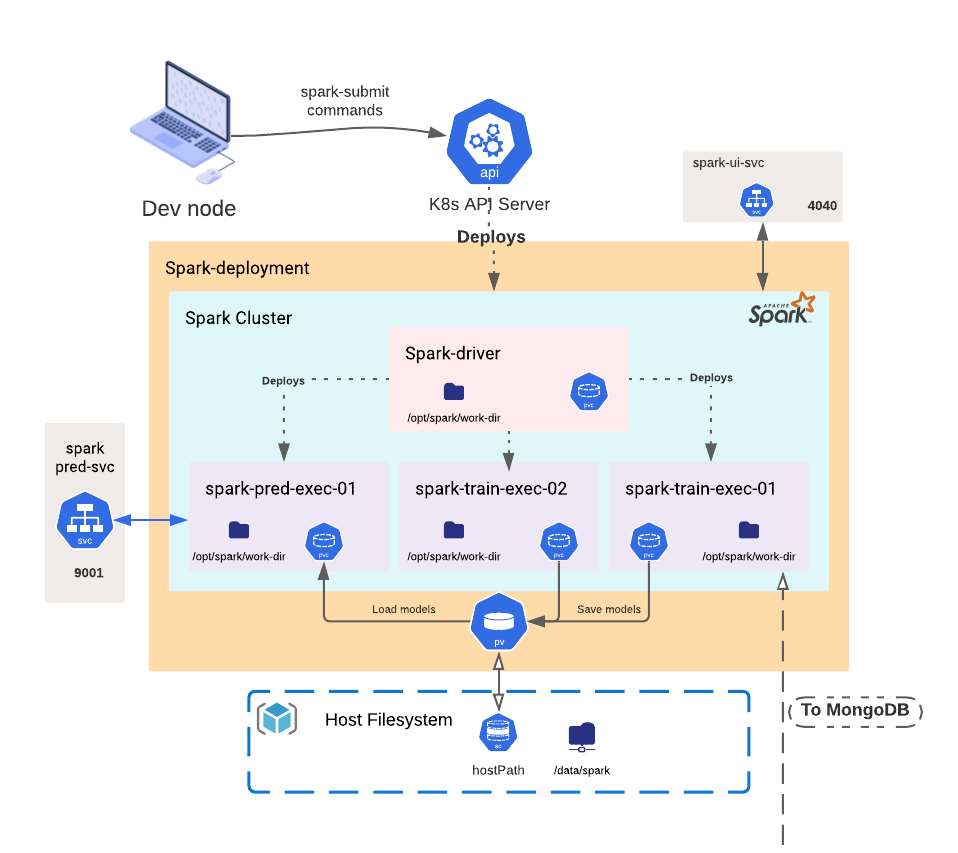
\includegraphics[width=0.9\linewidth]{imagenes/diagram-spark-kube.png}
	\caption{Spark on Kubernetes deployment architecture.}
	\label{diagram-spark-kube}
\end{figure}

\clearpage

\section{Additional Jobs and Modules}

In order to complete the Kubernetes deployment of the whole system, we created some additional items to automate some tasks and improve the reliability of the system over time. 

As we already mentioned in previous sections, we deployed a \textbf{Jupyter Notebook} environment for doing the data analysis and model comparison.

\begin{figure}[H]
	\centering
	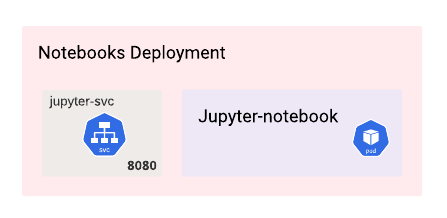
\includegraphics[width=0.6\linewidth]{imagenes/diagram-jupyter.png}
	\caption{Deployment and service architecure for the notebooks environment.}
	\label{diagram-jupyter}
\end{figure}

Additionally, we created two more resources to help us automate some tasks. Both items are what Kubernetes defines as Jobs or CronJobs, and are basically Pods that are deployed under certain conditions to complete a task, and then they are deleted.

The first Job will be a \textbf{data sink}. As the data we are using is exposed for one minute and then overriden by the new value in the Málaga Town Hall Open Data Portal, we need a way to keep a register of past values for training our model. 

We developed a Python script that scrapes the website and saves the data to our MongoDB database as a raw JSON. With the help of the Kubernetes CronJob resource and this script, we can save all the information in our database for future access, running the script every minute and logging the time of the download in the document metadata. 

For doing this, we created a light Docker image with the script loaded, and created the resource in Kubernetes so it runs every minute while the cluster is up. This is the way we acquired all the data used to train the model since the beginning of the development.

\begin{lstlisting}[language=yaml,caption=Kubernetes YAML definition file for the sink CronJob]
apiVersion: batch/v1
kind: CronJob
metadata:
  name: sink-job
  namespace: tfm
spec:
  schedule: "*/1 * * * *"
  jobTemplate:
    spec:
      template:
        spec:
          containers:
          - name: sink-job
            image: tonihurtado/sinkjob:latest
            imagePullPolicy: IfNotPresent
            command: ["python3", "/app/update-db.py"]
          restartPolicy: OnFailure
\end{lstlisting}
\label{section:Add}

The other CronJob, will have the task of running our training Job every month, with the new data scraped with the Sink Job. It will run on the first day of the month, and save the evaluation results on the storage so we can compare the performance of each model.


\chapter{Improvements and Future Work}
\label{chapter:Improvements}

The major shortcoming of this project has been the fact of not having a dataset large enough to perform an adequate training of the model, due to the non-existence of a register of past values by the entity providing the data in real-time. This led us not to obtain an accuracy value as good as we would have liked for our model. We have solved this problem by collecting the data ourselves, and as time goes by the size of the available dataset will increase, and with it, the evaluation parameters of the model will improve.

On the other hand, taking this deployment to a cloud service provider, even if it was a big challenge, would have been better in order to obtain a more realistic and robust system both for the Kubernetes cluster and, consequently, for Spark. This was not possible because the hardware resource requirements of our system design far exceeded those provided in the free plans of most platforms, even when student credits were provided.

Another improvement that could be really useful would have been to create a connector to be able to update the data of the public parking measurements directly to our context broker, through the implementation of an actuator. This would involve developing a service similar to the data sink, but that every time it reads the data from the source, it notifies Orion through the NGSIv2 API, providing it with the context information to be stored in our database through a Draco subscription. This could have helped us to integrate even more the system with the FIWARE components, and unify all the data flows through the Context Broker, but this solution required our cluster to be on for the whole time of the development of the project, so we decided to keep the data scraping service outside of the cluster.

Regarding tools and enhancements that could be added to improve the quality of the system, the Kubernetes configuration files could be moved to an infrastructure-as-code (IaS) tool, such as Terraform, which would allow us to add another layer of abstraction to our deployment. With this change, moving our system to a cloud service provider would be virtually automatic.

Also adding deployment automation and integration tools such as CircleCI or Jenkins would make the process of deploying our applications to the cluster automatic once we create a change in the Git repository. This is what is known as continuous integration, and its application is very interesting and useful in many use cases. 
\chapter{Conclusion}
\label{chapter:Conclusion}


Working on this project helped me to visualize many of the difficulties that developers and researchers encounter when facing the challenge of smart cities and the standardization of data, even if it is open data for public access. The fact of gathering data from such heterogeneous sources and systems generates the need to provide a context and a series of standard formats to this information so that automatic systems can process it. We have seen how FIWARE and the entire community formed around it is working to advance in this field and achieving very promising results.

On a personal level, I have also enjoyed the challenge of designing and managing a cluster with Kubernetes, and this project has also served to strengthen my knowledge of the technology and further reinforce my idea of working with similar systems in the future. It has also helped me to get to work with a real deployment of Machine Learning, and face similar problems that many people are facing right now with the boom of a technology as exciting as Artificial Intelligence.

In short, I think it has been a very transversal and complete project, where many of the technologies that have recently arrived to stay in our society, although they are invisible to the general public, have been addressed, and meanwhile, the problem of integrating them and creating a complete system has really helped me to understand their advantages and problems way better.

% Añadimos los apéndices que hagan falta
%\pdfbookmark[-1]{}{}
\appendix
\chapter{Code Snippets and Configuration files}

Here, I will place some of the scripts and configuration files mentioned during the development of the memory. They will be in appeareance order.

\textbf{Create Cluster Script}

\begin{lstlisting}[language=python, caption=Create Cluster script to automatically deploy the whole platform on minikube, label=CreateCluster]
#!/bin/bash
kubectl create namespace tfm
kubectl apply -f kubernetes/mongodb-sc.yaml
kubectl apply -f kubernetes/mongodb-statefulSet.yaml
echo "Starting database... [1m]"
sleep 60
echo "Configuring replicaset... [30s]"
sh statefulset/mongodb-rsconfig.sh mongodb-0
kubectl apply -f kubernetes/mongodb-hservice.yaml
echo "Starting mongodb UI... [1s]"
kubectl apply -f kubernetes/mongodb-express.yaml
sleep 10
echo "Starting context broker and draco (Fiware)... [5s]"
kubectl apply -f kubernetes/orion-service.yaml
kubectl apply -f kubernetes/orion-deployment.yaml
git clone https://github.com/ging/fiware-draco.git
kubectl apply -f kubernetes/draco-service.yaml
kubectl apply -f kubernetes/draco-deployment.yaml
sleep 10
echo "Starting Spark service account,volumes and services... [30s]"
kubectl create -n tfm serviceaccount spark
kubectl create -n tfm clusterrolebinding spark-role --clusterrole=edit --serviceaccount=tfm:spark --namespace=tfm
kubectl apply -f kubernetes/spark-pv.yaml
kubectl apply -f kubernetes/spark-pvc.yaml
kubectl apply -f kubernetes/spark-hservice.yaml
sleep 30
echo "Starting Web UI..."
kubectl apply -f kubernetes/prediction-web-deployment.yaml
sleep 2
echo "Running sink Job..."
kubectl apply -f kubernetes/Jobs/sink-job.yaml
sleep 5
echo "Creating ORION entities and subscriptions..."
pushd prediction-web/entities
sh curlEntities.sh
sleep 10
popd
echo "Submitting spark prediction Job..."
cd spark-job
mkdir -p spark-3.1.2 && curl -L https://dlcdn.apache.org/spark/spark-3.1.2/spark-3.1.2-bin-hadoop3.2.tgz | tar -zx -C spark-3.1.2/ --strip 1
sh spark-submit-predict.sh
sleep 20
echo "Done"
echo "Accessible services:"
minikube service list
\end{lstlisting}

\textbf{ReqTicketPrediction}

\begin{lstlisting}[language=json, caption=Definition file for the Orion entity that will define our requests tickets, label=ReqTicketPrediction]
{
    "id": "ReqTicketPrediction",
    "type": "ReqTicketPrediction",
    "predictionId": {
    "value": 0,
    "type": "String"
    },
    "socketId": {
    "value": 0,
    "type": "String"
    },
    "name":{
    "value": 0,
    "type": "String"
    },
    "year":{
    "value": 0,
    "type": "Int"
    },
    "month":{
    "value": 0,
    "type": "Int"
    },
    "day":{
    "value": 0,
    "type": "Int"
    },
    "weekday": {
    "value": 0,
    "type": "Integer"
    },
    "time": {
    "value": 0,
    "type": "Integer"
    }
}
\end{lstlisting}

\textbf{ResTicketPrediction}

\begin{lstlisting}[language=json, caption=Definition file for the Orion entity that will define our response tickets, label=ResTicketPrediction]
{
    "id": "ResTicketPrediction",
    "type": "ResTicketPrediction",
    "predictionId": {
        "value": "0",
        "type": "String"
    },
    "socketId": {
        "value": 0,
        "type": "String"
    },
    "predictionValue":{
        "value": 0,
        "type": "Integer"
    },
    "name":{
        "value": 0,
        "type": "String"
    },
    "weekday":{
        "value": 0,
        "type": "Integer"
    },
    "time": {
        "value": 0,
        "type": "Integer"
    }
}
\end{lstlisting}

\textbf{subscribeReqPredictionTicket}:

\begin{lstlisting}[language=json, caption=Definition file for the Orion subscription that will trigger the predictions on Spark, label=subscribeReqPredictionTicket]
{
    "description": "A subscription to get ticket predictions",
    "subject": {
        "entities": [
        {
            "id": "ReqTicketPrediction",
            "type": "ReqTicketPrediction"
        }
        ],
        "condition": {
        "attrs": [
        "predictionId"
        ]
        }
    },
    "notification": {
        "http": {
        "url": "http://spark-predict-svc:9001"
        },
        "attrs": [
        "predictionId",
        "socketId",
        "name",
        "year",
        "month",
        "day",
        "weekday",
        "time"
        ]
    },
    "expires": "2040-01-01T14:00:00.00Z",
    "throttling": 5
}
\end{lstlisting}


\textbf{subscribeResPredictionTicket}:

\begin{lstlisting}[language=json, caption=Definition file for the Orion subscription that will trigger the response to the webapp., label=subscribeResPredictionTicket]
{
    "description": "A subscription to get ticket predictions",
    "subject": {
        "entities": [
        {
            "id": "ResTicketPrediction",
            "type": "ResTicketPrediction"
        }
        ],
        "condition": {
        "attrs": [
        "predictionId"
        ]
        }
    },
    "notification": {
        "http": {
        "url": "http://web-service:3000/notify"
        },
        "attrs": [
        "predictionId",
        "socketId",
        "predictionValue",
        "name",
        "weekday",
        "time"
        ]
    },
    "expires": "2040-01-01T14:00:00.00Z",
    "throttling": 5
}
\end{lstlisting}

\textbf{subscribeResDracoPredictionTicket}:

\begin{lstlisting}[language=json, caption=Definition file for the Orion subscription that will trigger Draco por processing., label=subscribeResDracoPredictionTicket]
{
    "description": "A subscription to get ticket predictions",
    "subject": {
      "entities": [
        {
          "id": "ResTicketPrediction",
          "type": "ResTicketPrediction"
        }
      ],
      "condition": {
        "attrs": [
        "predictionId",
        "socketId",
        "predictionValue",
        "name",
        "weekday",
        "time"
        ]
      }
    },
    "notification": {
      "http": {
        "url": "http://draco:5050/v2/notify"
      },
      "attrs": [
        "predictionId",
        "socketId",
        "predictionValue",
        "name",
        "weekday",
        "time"
      ]
    },
    "expires": "2040-01-01T14:00:00.00Z",
    "throttling": 5
}
\end{lstlisting}

\textbf{MongoDB Kubernetes StatefulSet}

\begin{lstlisting}[language=yaml,caption=Kubernetes YAML definition file for MongoDB StatefulSet Deployment, label=MongoKubernetes]
apiVersion: apps/v1
kind: StatefulSet
metadata:
    name: mongodb
    namespace: tfm
spec:
    serviceName: mongodb-svc
    replicas: 3
    selector:
    matchLabels:
        app: db
        name: mongodb
    template:
    metadata:
        namespace: tfm
        labels:
        app: db
        name: mongodb
        replicaset: MainRepSet
    spec:
        terminationGracePeriodSeconds: 10
        containers:
        - name: mongo
            image: mongo
            command:
            - "mongod"
            - "--bind_ip"
            - "0.0.0.0"
            - "--replSet"
            - "MainRepSet"
            resources:
            requests:
                cpu: 0.2
                memory: 200Mi
            ports:
            - containerPort: 27017
            volumeMounts:
            - name: mongodb-persistent-storage-claim
                mountPath: /data/db
    volumeClaimTemplates:
    - metadata:
        name: mongodb-persistent-storage-claim
    spec:
        storageClassName: mongodb
        accessModes: [ "ReadWriteOnce" ]
        resources:
        requests:
            storage: 1Gi
\end{lstlisting}

\textbf{Orion Kubernetes Deployment and Service}:

\begin{lstlisting}[language=yaml,caption=Kubernetes YAML definition file for Orion Deployment, label=OrionKubernetes]
    apiVersion: apps/v1
    kind: Deployment
    metadata:
        labels:
        service: orion
        name: orion
        namespace: tfm
    spec:
        replicas: 1
        selector:
        matchLabels:
            service: orion
        template:
        metadata:
            namespace: tfm
            labels:
            service: orion
        spec:
            containers:
            - args: ["-dbhost","mongodb-svc:27017","-rplSet","MainRepSet","-logLevel","DEBUG","-httpTimeout","15000","-dbDisableRetryWrites","-port","1026"] 
                image: fiware/orion
                name: orion
                ports:
                - containerPort: 1026
            restartPolicy: Always
\end{lstlisting}


\begin{lstlisting}[language=yaml,caption=Kubernetes YAML definition file for Orion Service, label=OrionKubernetesService]
    apiVersion: v1
    kind: Service
    metadata:
      namespace: tfm
      labels:
        service: orion
      name: orion
    spec:
      type: NodePort
      ports:
        - port: 1026
          targetPort: 1026
          nodePort: 30329
      selector:
        service: orion
\end{lstlisting}

\textbf{Draco Kubernetes Deployment and Service}:

\begin{lstlisting}[language=yaml,caption=Kubernetes YAML definition file for Draco Deployment., label=DracoKubernetes]
    apiVersion: apps/v1
    kind: Deployment
    metadata:
        labels:
        service: draco
        name: draco
        namespace: tfm
    spec:
        replicas: 1
        selector:
        matchLabels:
            app: draco
        template:
        metadata:
            namespace: tfm
            labels:
            app: draco
        spec:
            containers:
            - name: draco
            image: tonihurtado/draco:latest
            imagePullPolicy: Always
            restartPolicy: Always
\end{lstlisting}

\begin{lstlisting}[language=yaml,caption=Kubernetes YAML definition file for Draco Service., label=DracoKubernetesService]
apiVersion: v1
kind: Service
metadata:
    namespace: tfm
    labels:
    service: draco  
    name: draco
spec:
    type: NodePort
    ports:
    - port: 5050
        targetPort: 5050
        name: data
    - port: 8080
        targetPort: 8080
        name: ui
    selector:
    app: draco
\end{lstlisting}
\thispagestyle{empty}

% Añadimos la bibliografia
\nocite{}
\bibliographystyle{IEEEtran}
\bibliography{bibliografia/bibliography.bib}

\addcontentsline{toc}{chapter}{Bibliografía}


\end{document}
